\subsection{Optimization Methodology}
\begin{frame}
    \frametitle{AHTR Optimization Problem Definitions}
    \vspace{-0.2cm}
    \visible<1->{\begin{block}{Varied Input Parameters}
        \begin{itemize}
            \item Total fuel packing fraction ($PF_{total}$)
            \item TRISO fuel packing fraction distribution ($\rho_{TRISO}(\vec{r})$)
            \item Coolant channel shape ($r_i$)
        \end{itemize}}
        \visible<2->{Varying $PF_{total}$ and $\rho_{TRISO}(\vec{r})$ synergistically 
        explores how \textbf{heterogenous TRISO distribution could minimize 
        self-shielding} and thus, reduce the fuel required.}
    \end{block}
    \vspace{-0.3cm}
    \visible<3->{\begin{block}{AHTR Optimization Objectives}
     \textbf{Minimize total fuel packing fraction ($PF_{total}$)}
     \begin{itemize}
        \item Cost savings, non-proliferation 
     \end{itemize}
     \textbf{Minimize maximum temperature ($T_{max}$)}
     \begin{itemize}
        \item Minimize thermal stress in the fuel 
     \end{itemize}
     \textbf{Minimize fuel-normalized power peaking factor ($PPF_{fuel}$)} 
     \begin{itemize}
        \item Efficient fuel utilization
     \end{itemize}
    \end{block}}
    \visible<4->{\textbf{I optimized the AHTR plank and one-third assembly geometries.}} 
\end{frame}

\begin{frame}
    \frametitle{AHTR One-Third Assembly Geometry}
    \begin{columns}[t]
        \begin{column}{0.5\textwidth}
        \vspace{0.1cm}
        \visible<1->{\textbf{Two sine distributions govern TRISO packing fraction 
        distribution:}
        \vspace{-0.2cm} 
        \begin{align}
        \rho_{TRISO}(\vec{x}, \vec{y}) &= \left(\textbf{a}\cdot sin(\textbf{b}\cdot 
        x + \textbf{c}) + 2\right) \nonumber \\
        & \cdot \left(\textbf{d}\cdot sin(\textbf{e}\cdot y + \textbf{f}) + 2\right) 
        \cdot NF \nonumber
        \end{align}
        \vspace{-0.7cm}
        \begin{figure}
            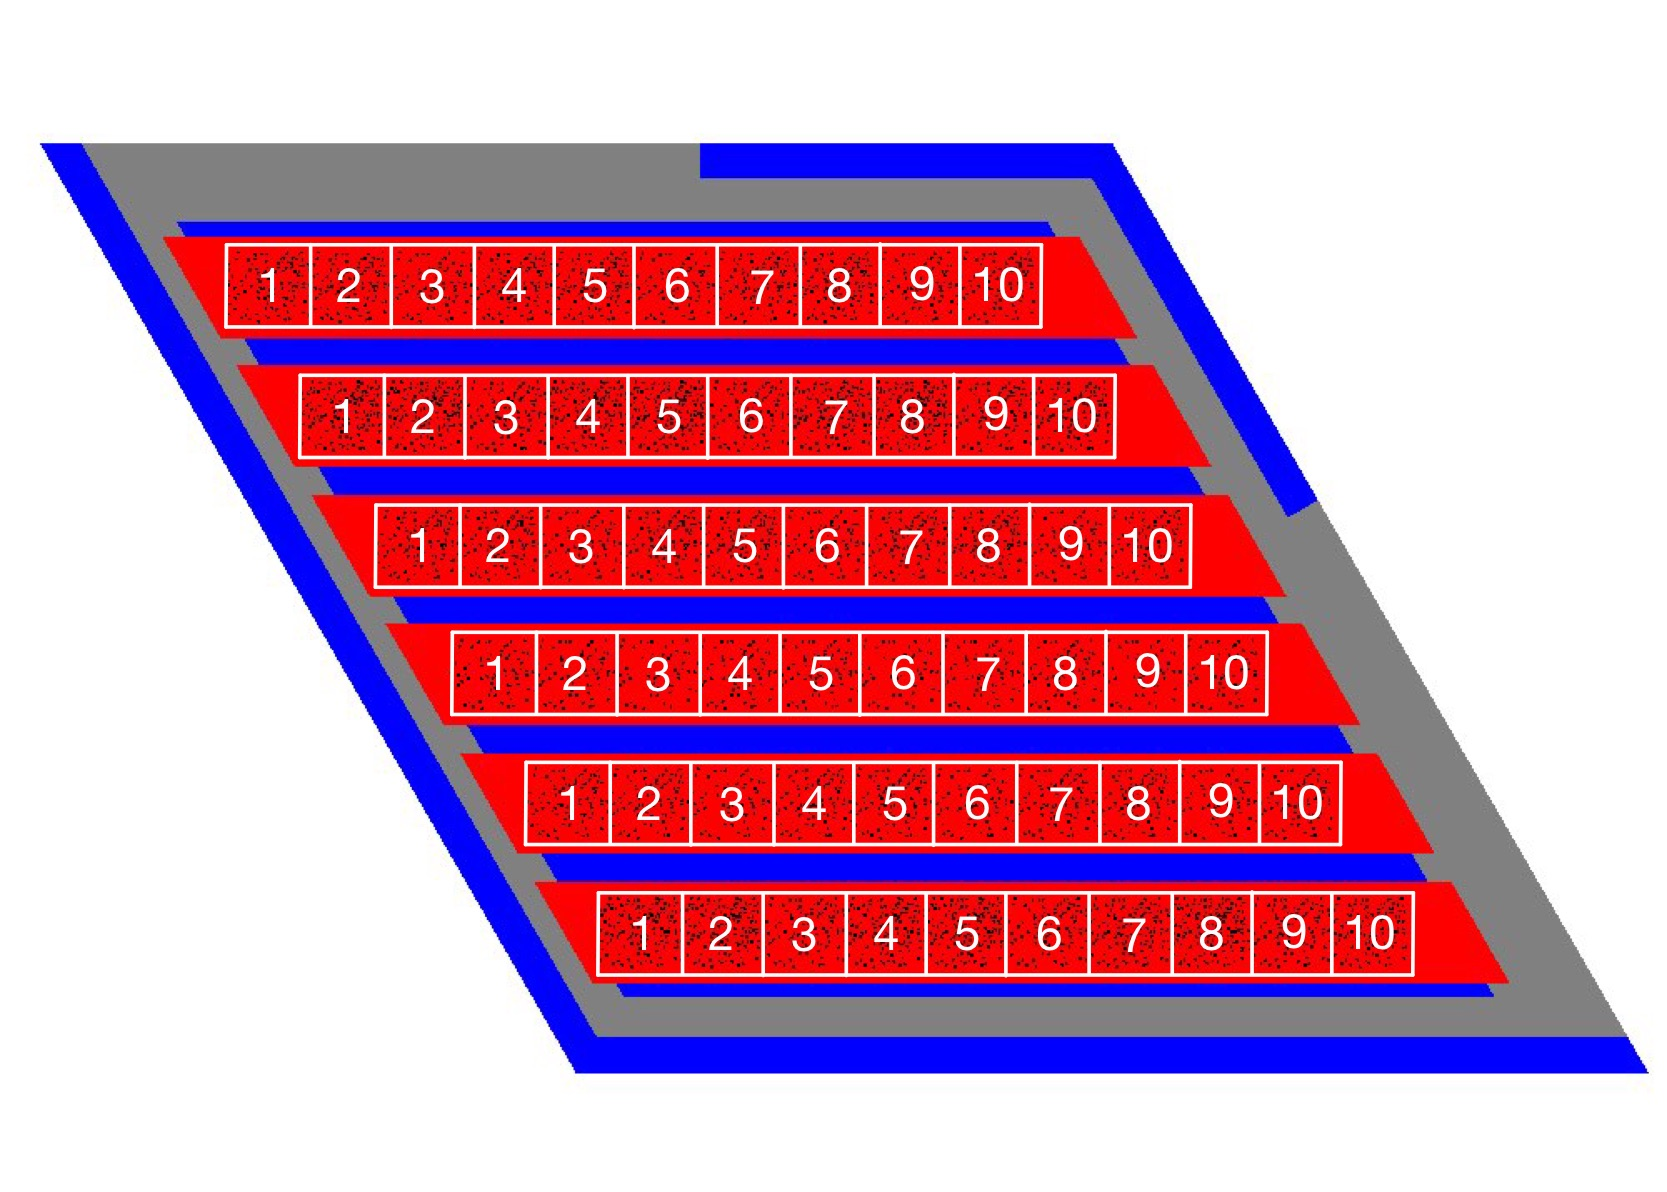
\includegraphics[width=\linewidth]{../docs/figures/ahtr_assembly.png} 
            \caption{AHTR one-third assembly with ten randomly packed fuel cells in 
            each graphite plank.}
        \end{figure}}
        \end{column}
        \begin{column}{0.5\textwidth} 
            \visible<2->{\textbf{Five radius values (\textbf{$r_1, r_2, r_3, r_4, r_5$}) 
            control coolant channel shape.}
            \begin{figure}
                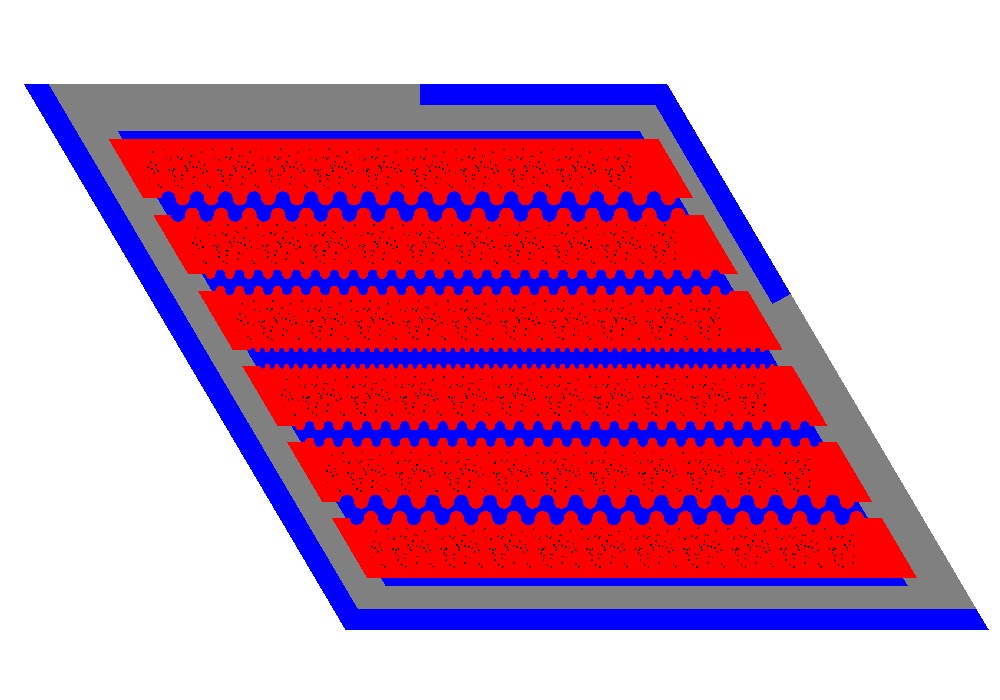
\includegraphics[width=\linewidth]{../docs/figures/coolant-channel-shape-assem.png} 
                \caption{AHTR one-third assembly with coolant channel shape variation, 
                $r_1, r_2, r_3, r_4, r_5$ = 0.3cm, 0.2cm, 0.1cm, 0.2cm, 0.3cm.}
            \end{figure}}
        \end{column}
        \end{columns}
\end{frame}

\begin{frame}
    \frametitle{ROLLO AHTR Optimization Workflow}
    \vspace{-0.2cm}
    \begin{figure}
        \makebox[\textwidth][c]{
            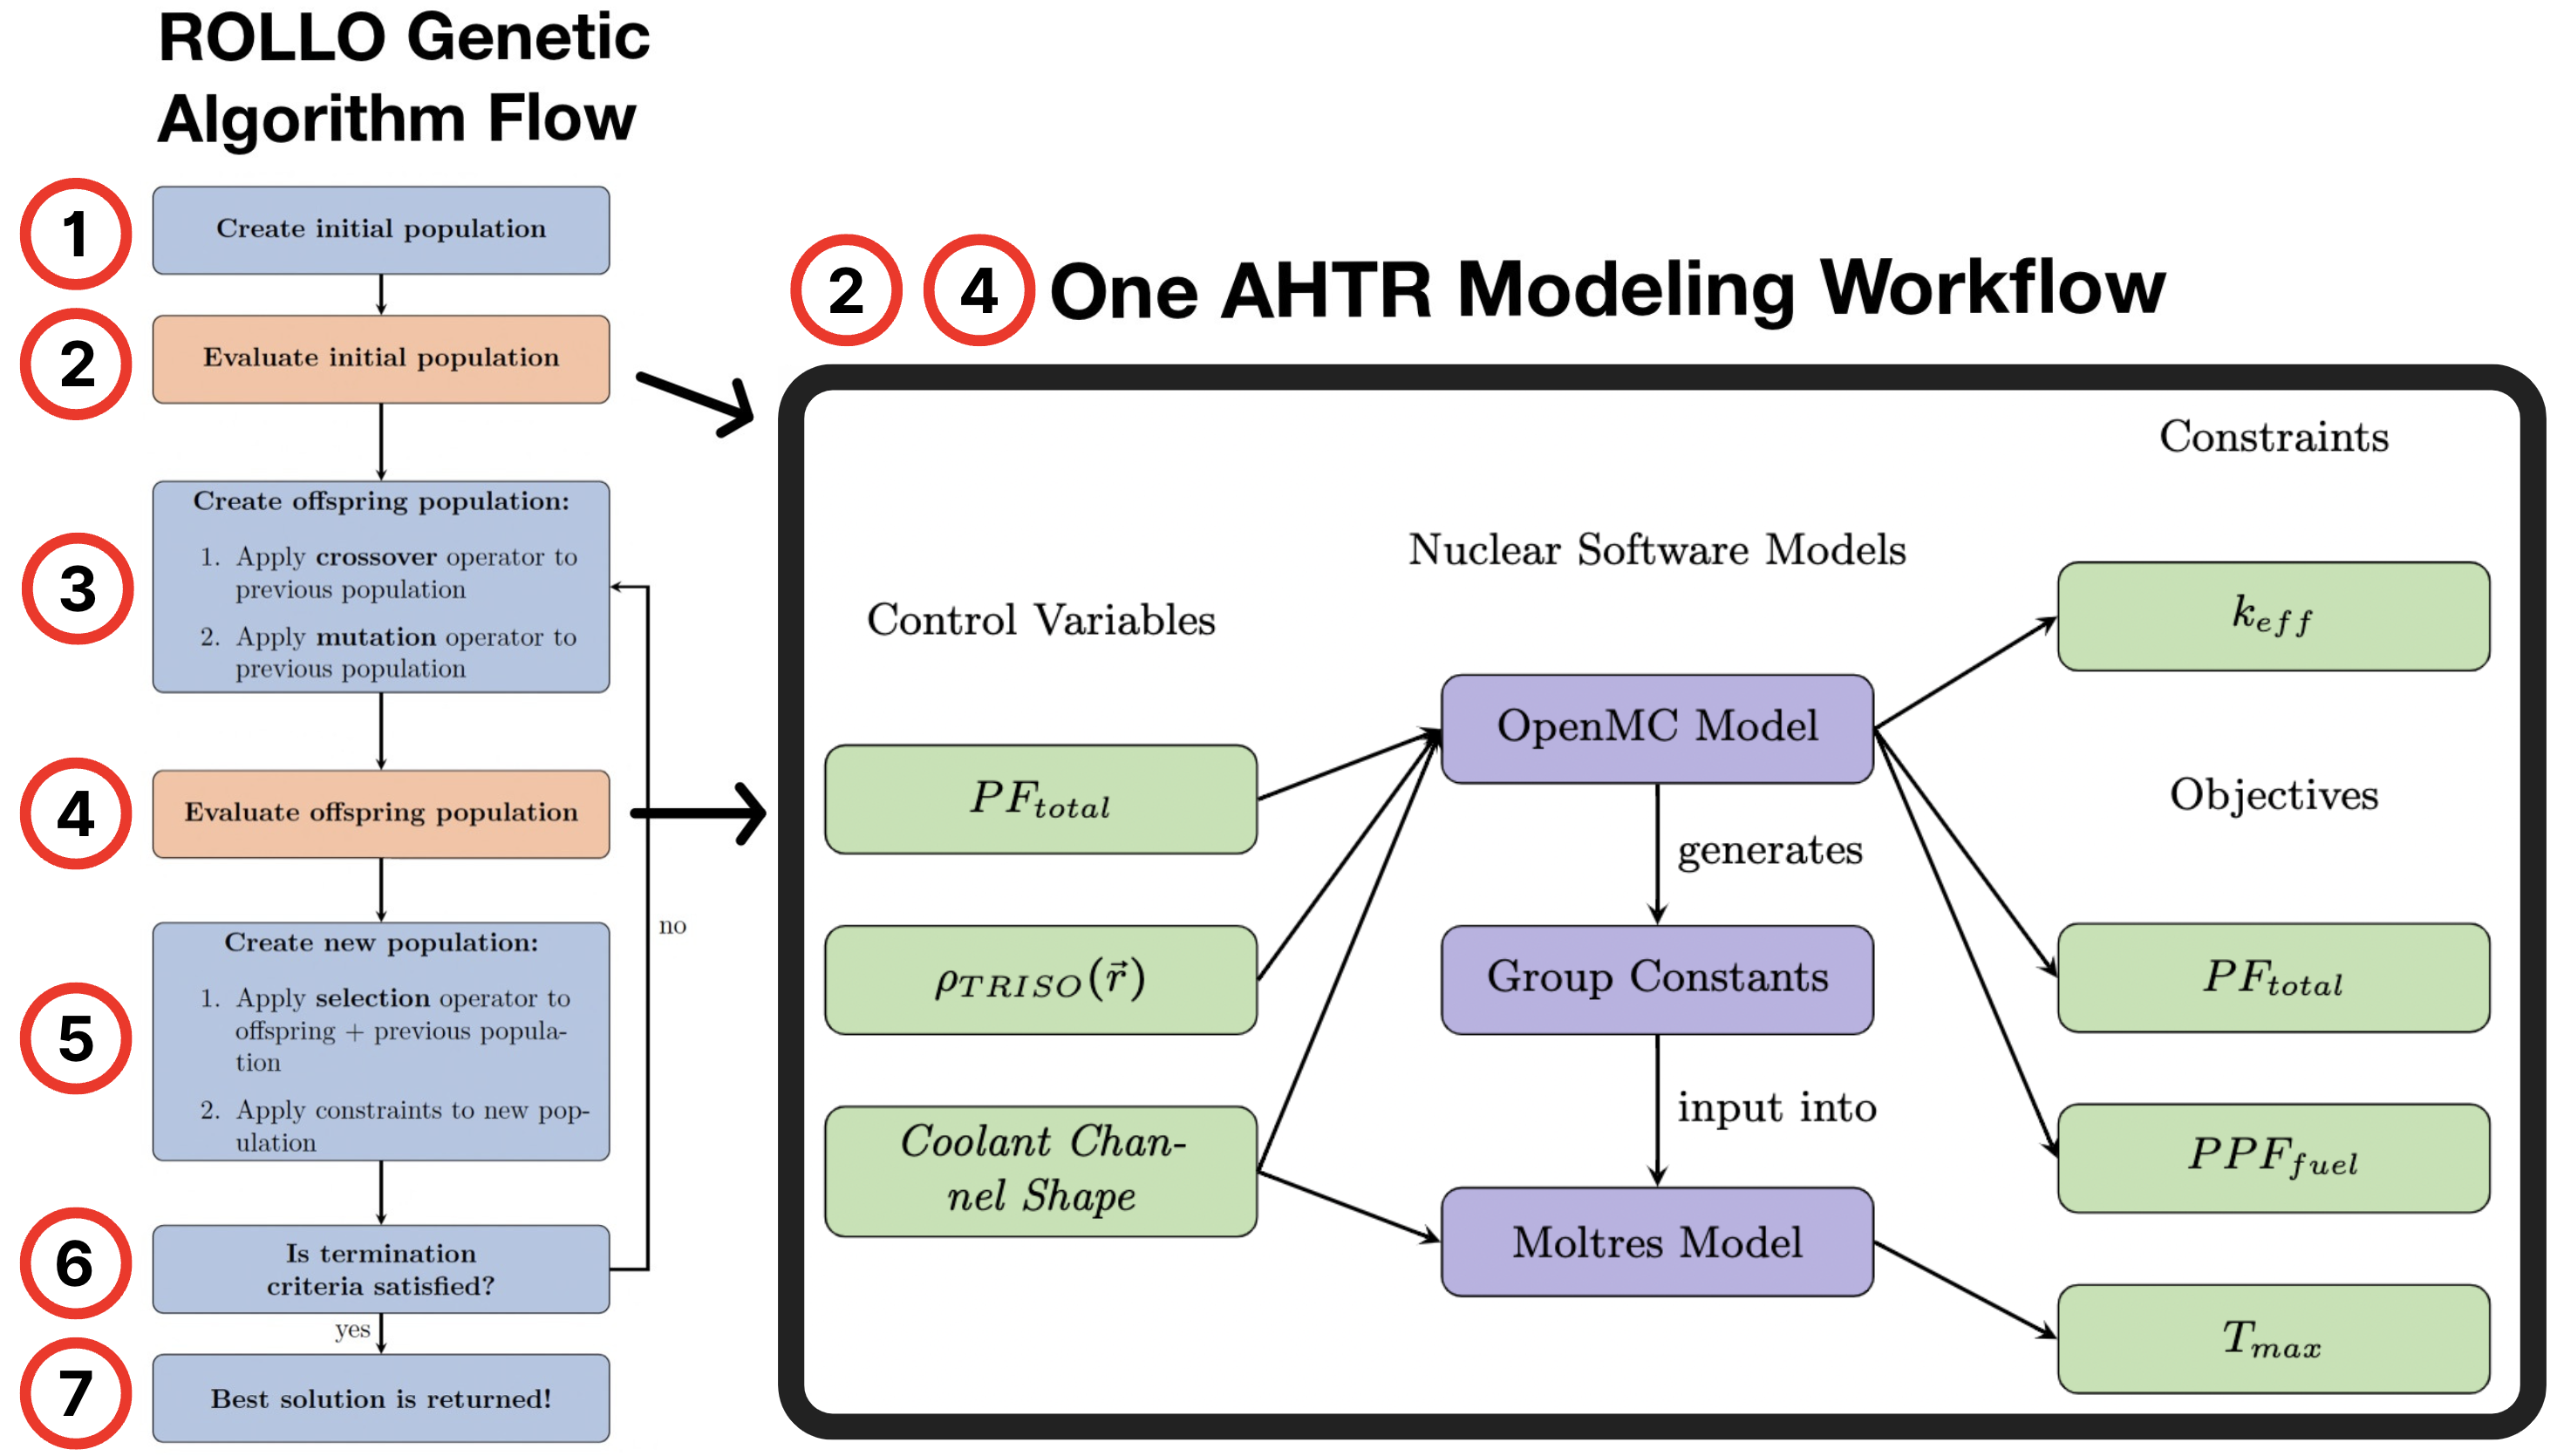
\includegraphics[width=1.18\linewidth]{figures/ahtr-modeling-workflow-numbered.png}} 
        %\caption{ROLLO AHTR Optimization Workflow.}
    \end{figure}
\end{frame}

\subsection{AHTR One-Third Assembly Optimization Results}
\begin{frame}
    \frametitle{AHTR One-Third Assembly Optimization Simulations}
    \only<1>{
        \vspace{-0.2cm}
        \begin{figure}
            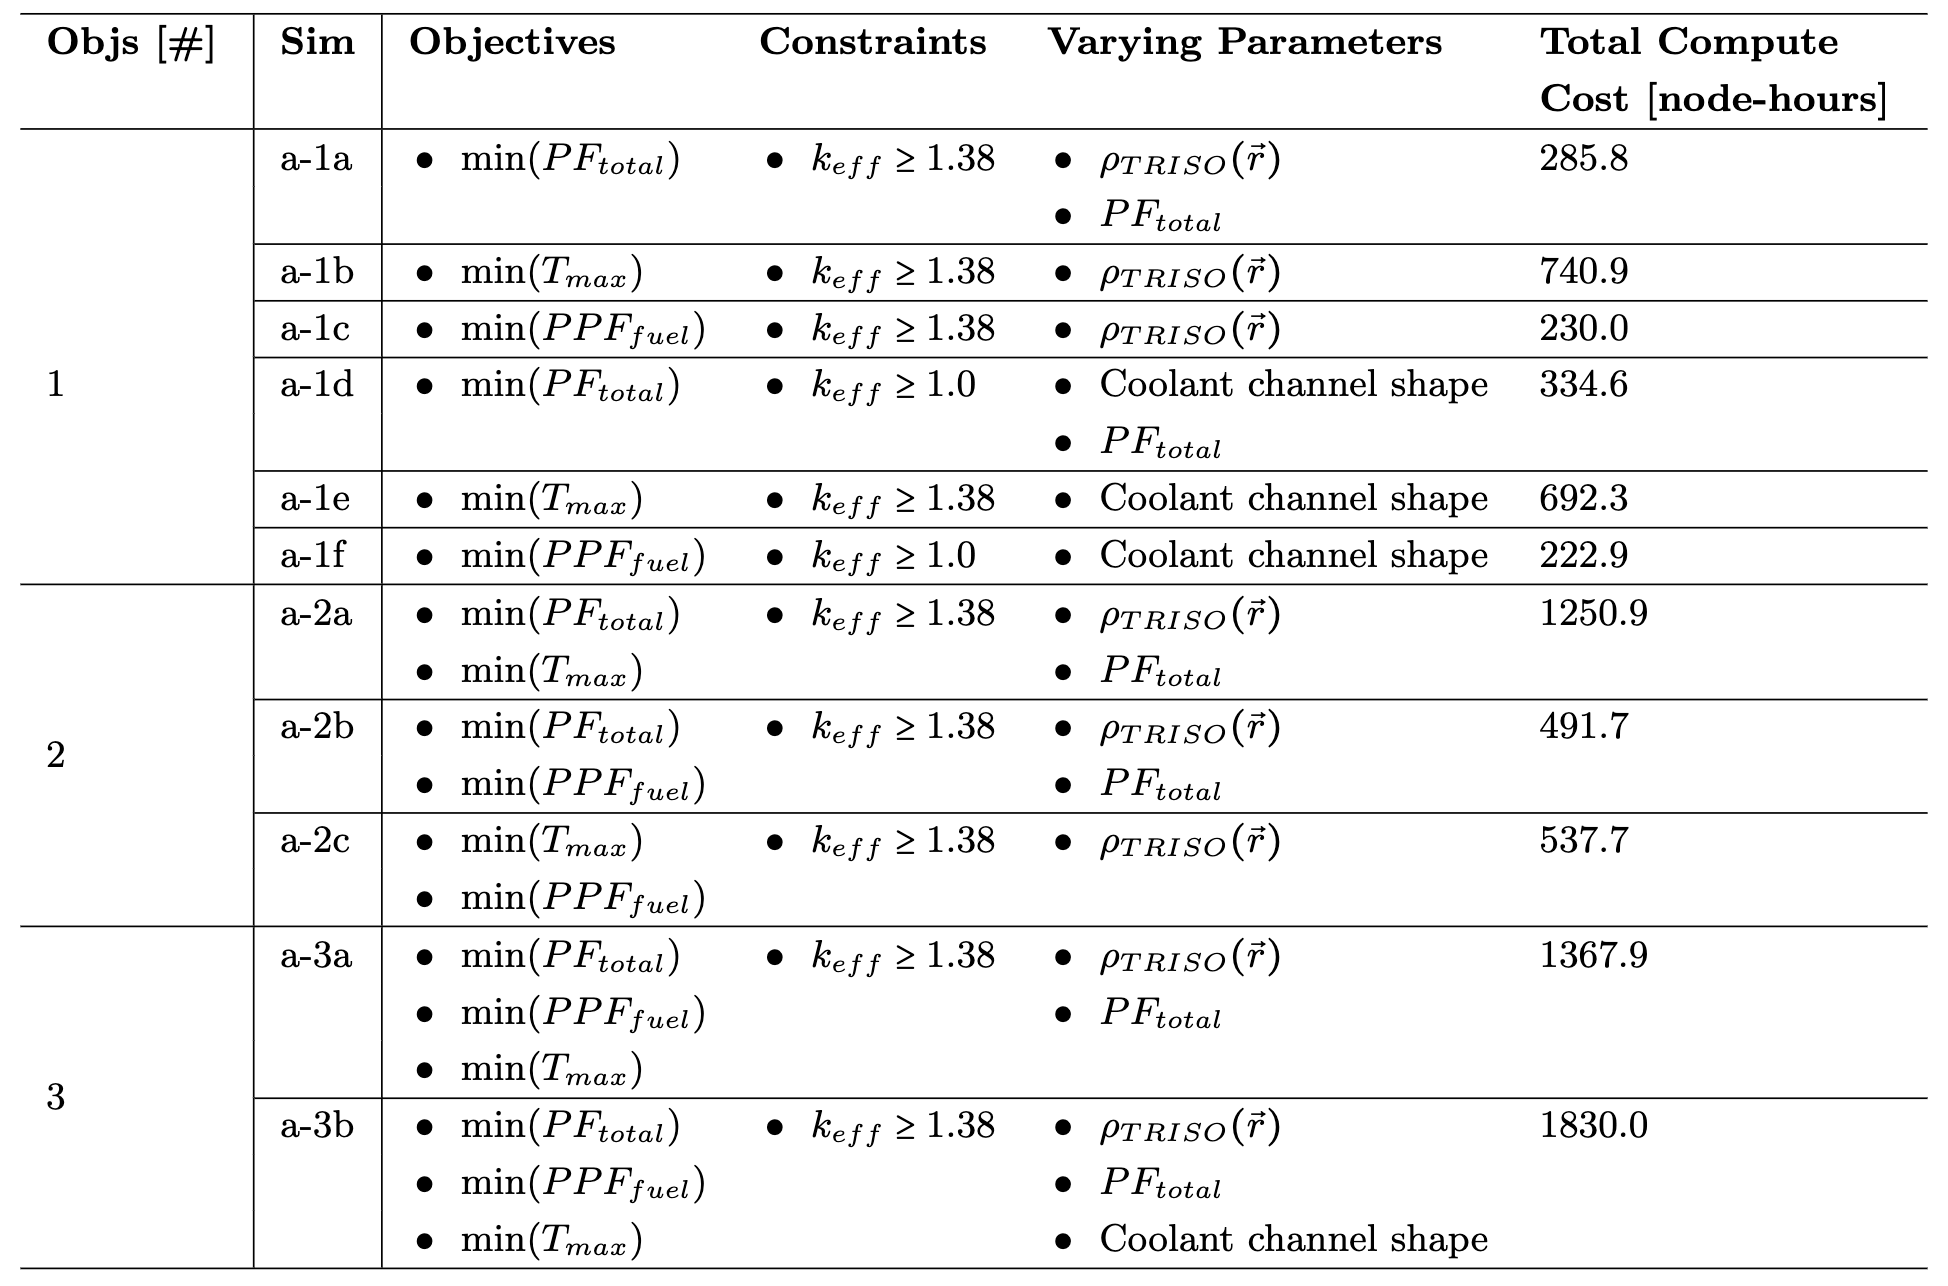
\includegraphics[width=0.8\linewidth]{figures/ahtr-assem-opt-table.png}
        \end{figure}

        \vspace{-0.2cm}
        All the optimization simulations are run on the \textbf{Theta supercomputer} 
        at the Argonne Leadership Computing Facility \cite{noauthor_thetathetagpu_2022}.

        Each Theta node has 64 1.3-GHz Intel Xeon Phi 7230 processors.}
        \only<2>{
            \begin{figure}
                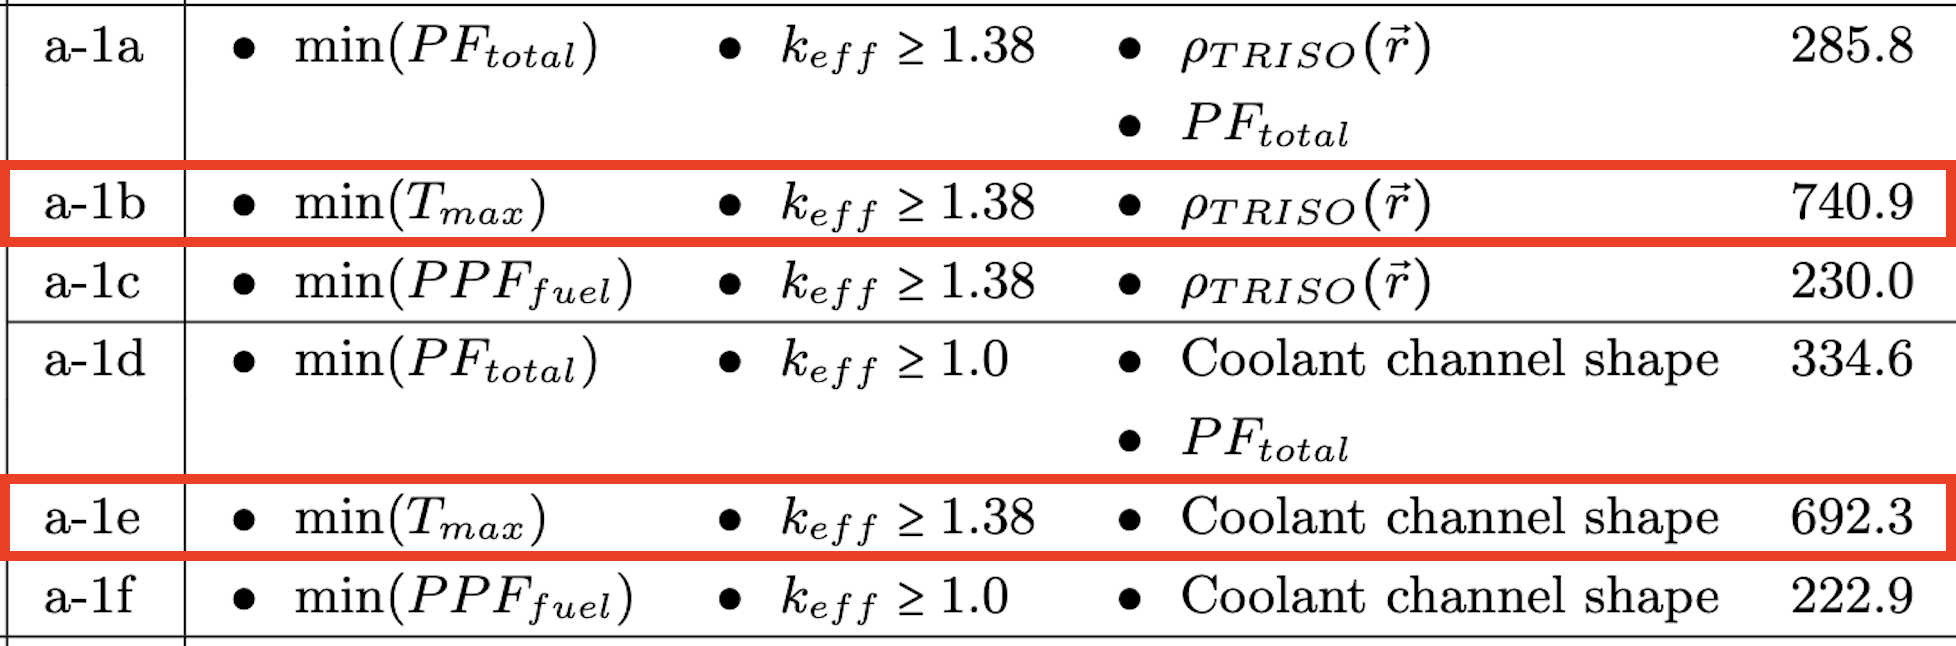
\includegraphics[width=\linewidth]{figures/ahtr-assem-opt-table-annotated1.png}
            \end{figure}
    
            Simulations a-1b and a-1e demonstrate \textbf{how the $\rho_{TRISO}(\vec{r})$ 
            and coolant channel shape varying parameters respond to 
            the minimize $T_{max}$ objective}.

            \vspace{0.2cm}
            I constrained $k_{eff} \geq 1.38$ find optimal input parameters 
            that achieve \textbf{similar performance to the FHR benchmark} TRISO distribution.}
        
        \only<3>{
            \begin{figure}
                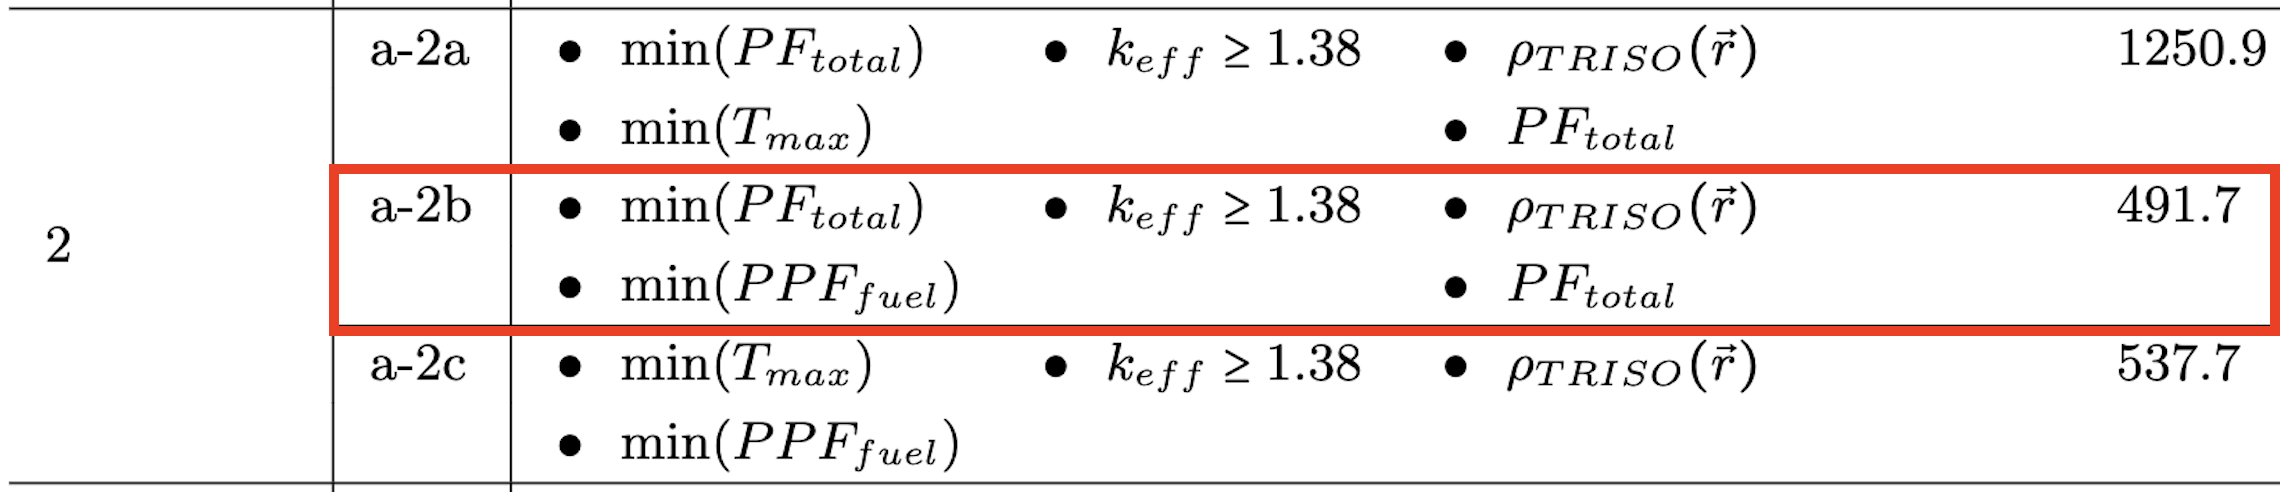
\includegraphics[width=\linewidth]{figures/ahtr-assem-opt-table-annotated2.png}
            \end{figure}

            Simulation a-2b demonstrates how input parameters $PF_{total}$ and 
            $\rho_{TRISO}(\vec{r})$ change as the minimize $PF_{total}$ and $PPF_{fuel}$ 
            objectives interact.
        }

        \only<4>{
            \begin{figure}
                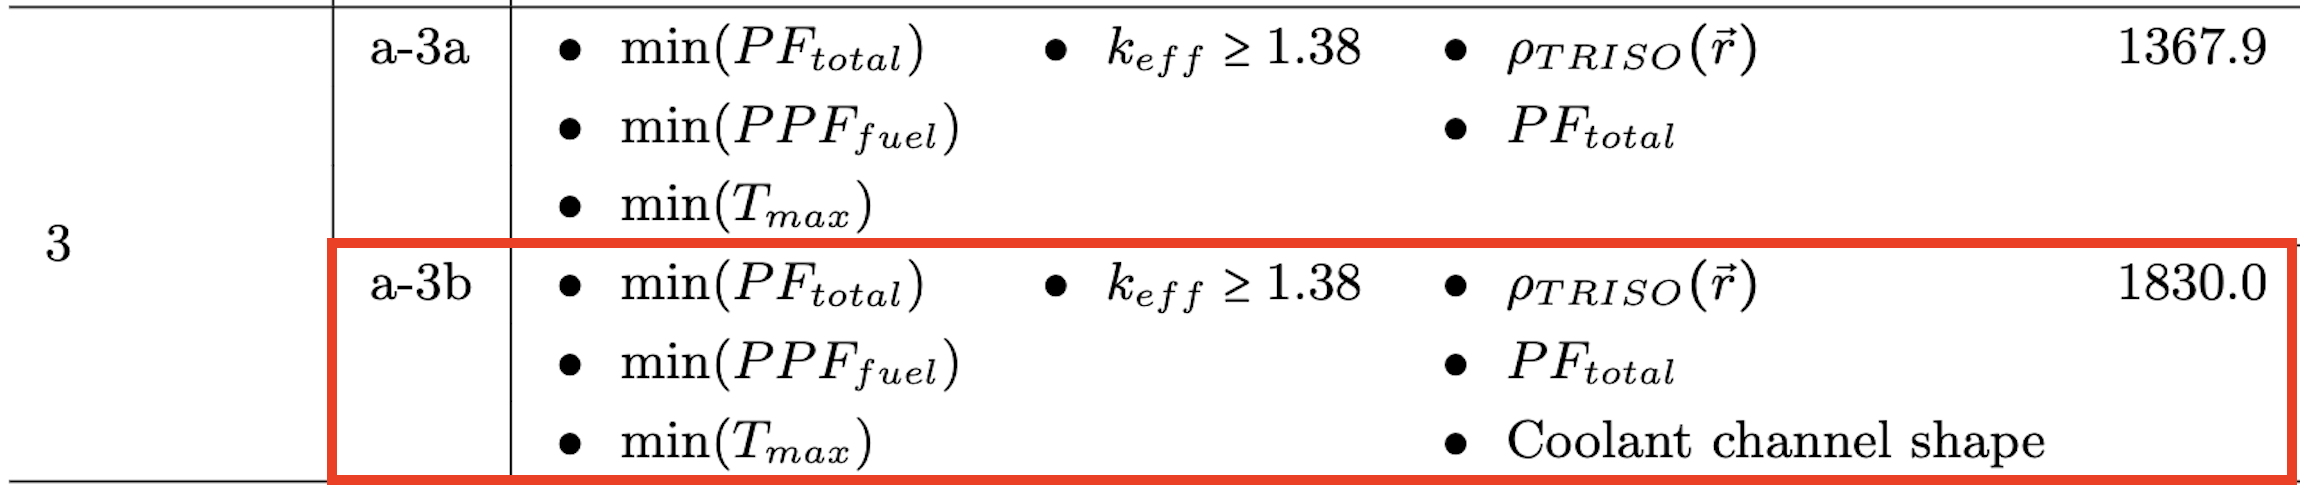
\includegraphics[width=\linewidth]{figures/ahtr-assem-opt-table-annotated3.png}
            \end{figure}

            Simulation a-3b is the \textbf{final and largest optimization problem} run for 
            the one-third assembly model that varies all input parameters to optimize 
            for all objectives. 
        }
    
\end{frame}

\begin{frame}
    \frametitle{AHTR One-Third Assembly Simulation a-1b Results}
    I vary \textbf{a, b, c, d, e f} ($\rho_{TRISO}(\vec{x}, \vec{y}$))
    to minimize $T_{max}$. 

    \begin{figure}
        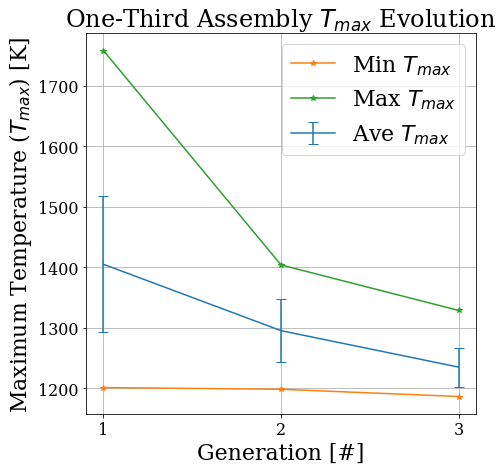
\includegraphics[width=0.39\linewidth]{figures/assem-obj-1-temp-evol-pres.png} 
        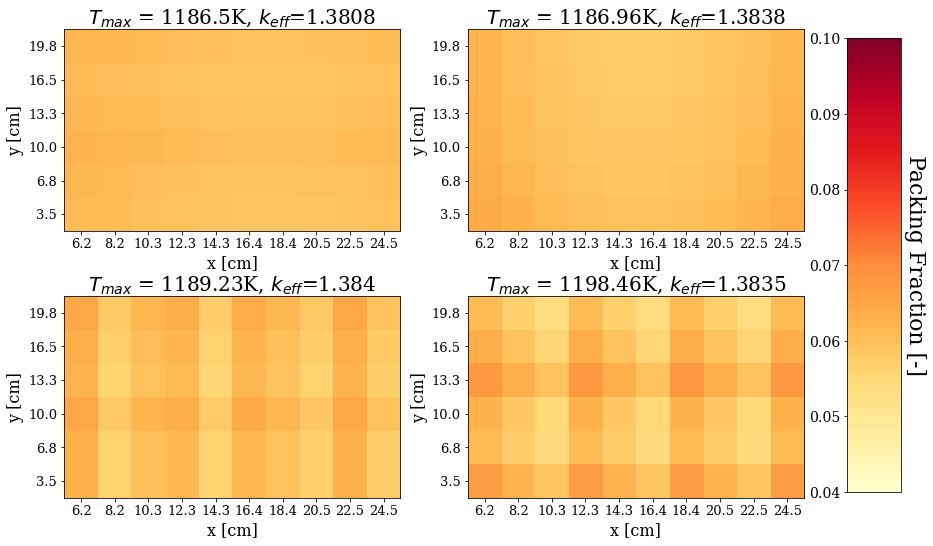
\includegraphics[width=0.59\linewidth]{../docs/figures/assem-obj-1-temp-final.png}
        \caption{Simulation a-1b $T_{max}$ evolution.}
    \end{figure}

    \begin{tcolorbox}[colback=illiniorange,colframe=illiniorange!50!black]
        \textbf{A flatter TRISO distribution minimizes $T_{max}$.}
    \end{tcolorbox}
\end{frame}

\begin{frame}
    \frametitle{AHTR One-Third Assembly Simulation a-1e Results}
    I vary $r_1, r_2, r_3, r_4, r_5$ (coolant channel shape)
    to minimize $T_{max}$. 
    \begin{figure}
        \centering
        \begin{subfigure}{0.3\textwidth}
            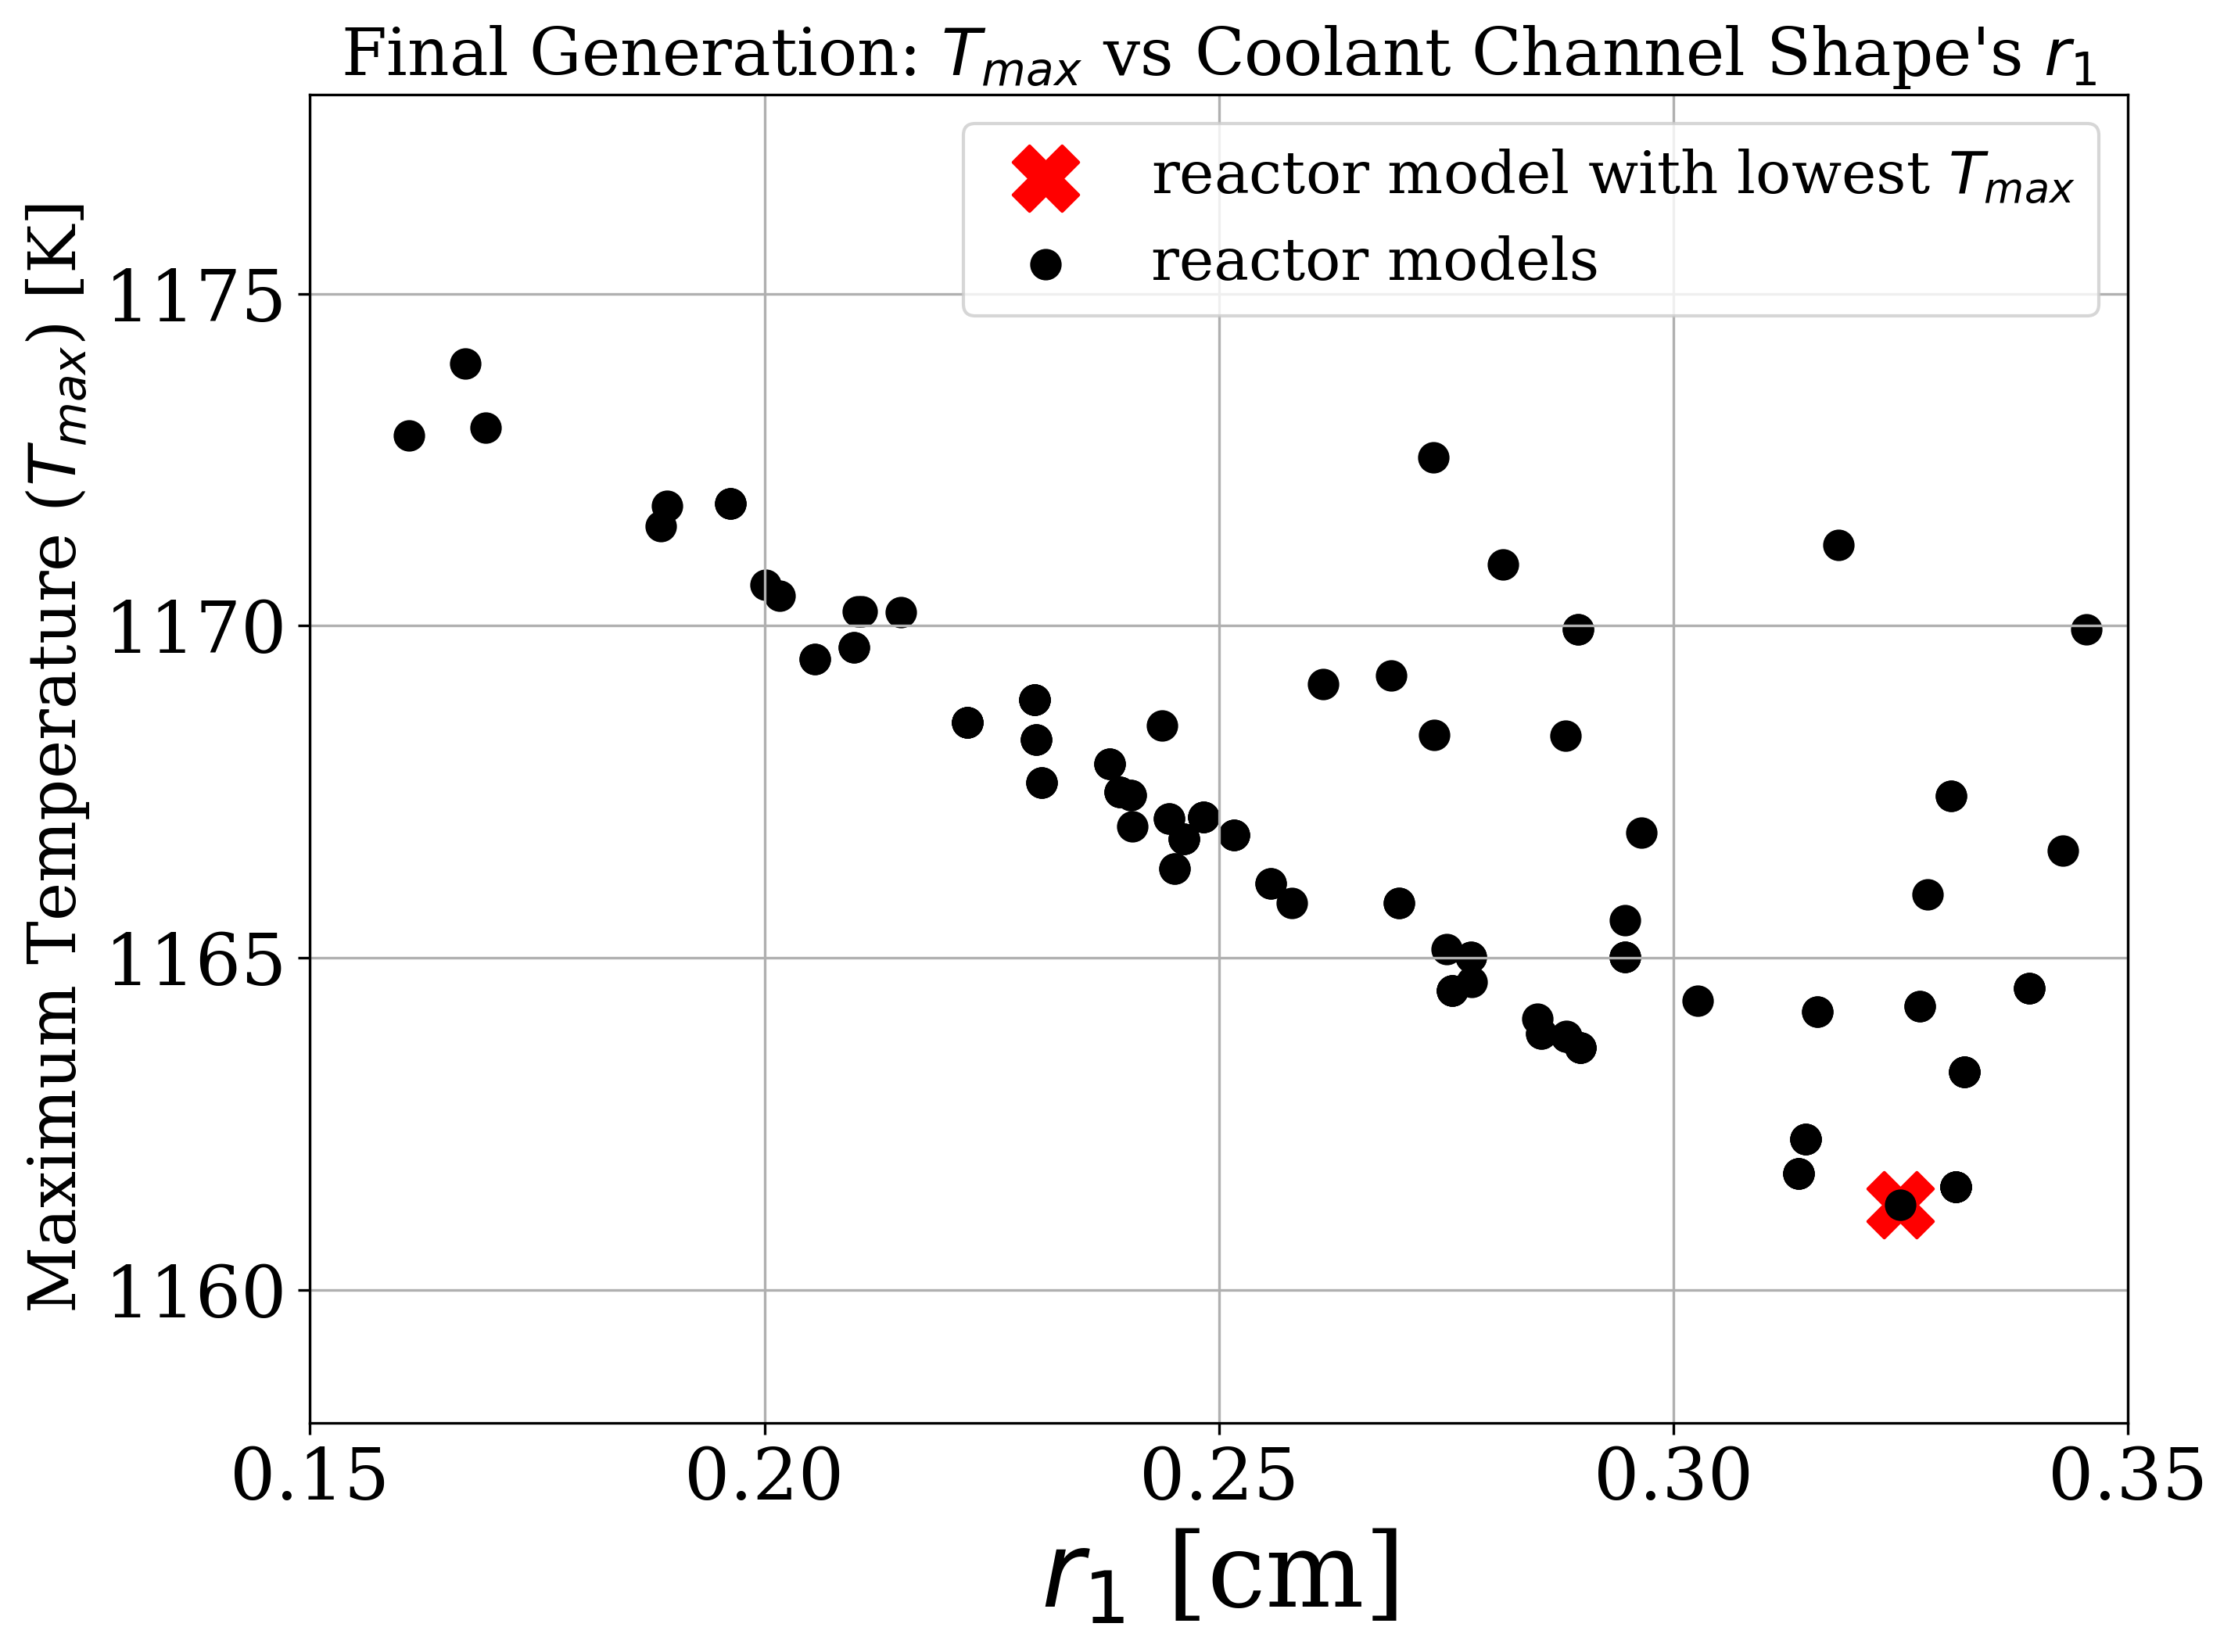
\includegraphics[width=\linewidth]{figures/a-1e-r1-pres.png}
            \caption{Plot of $T_{max}$ against $r_1$.}
            \label{fig:a-1e-r1} 
        \end{subfigure}
        \begin{subfigure}{0.3\textwidth}
            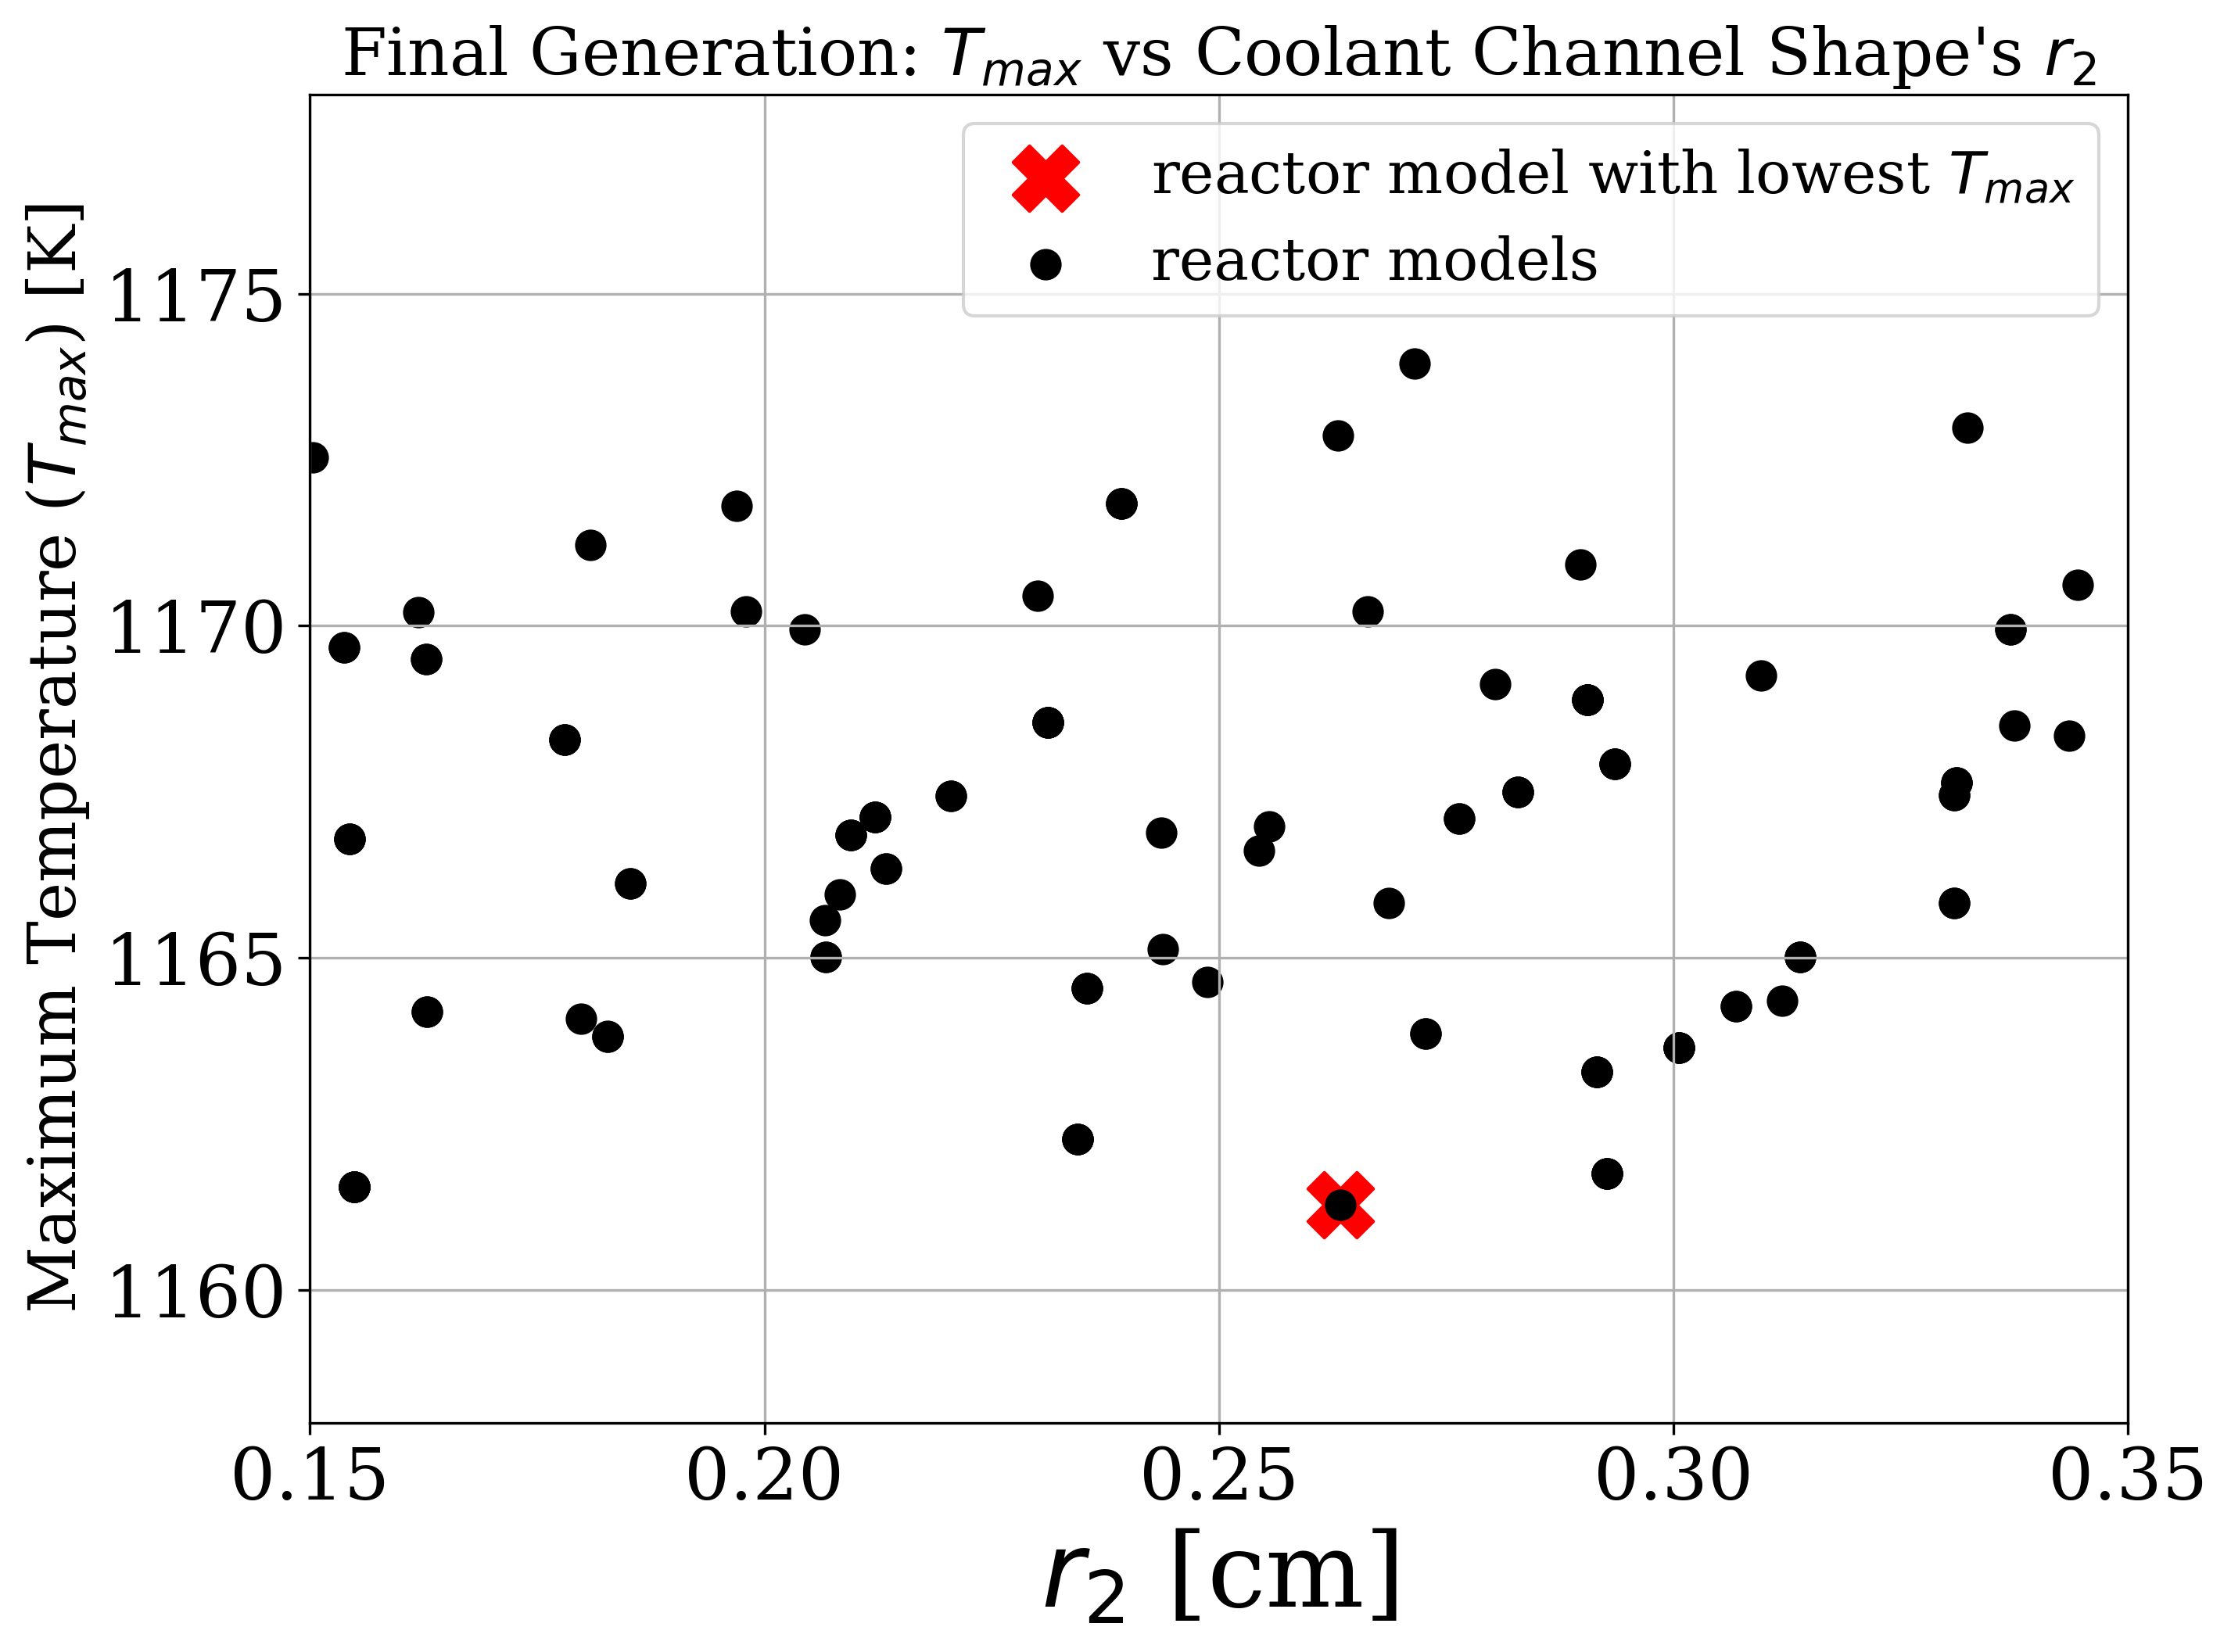
\includegraphics[width=\linewidth]{figures/a-1e-r2-pres.png}
            \caption{Plot of $T_{max}$ against $r_2$.}
            \label{fig:a-1e-r2} 
        \end{subfigure}
        \begin{subfigure}{0.3\textwidth}
            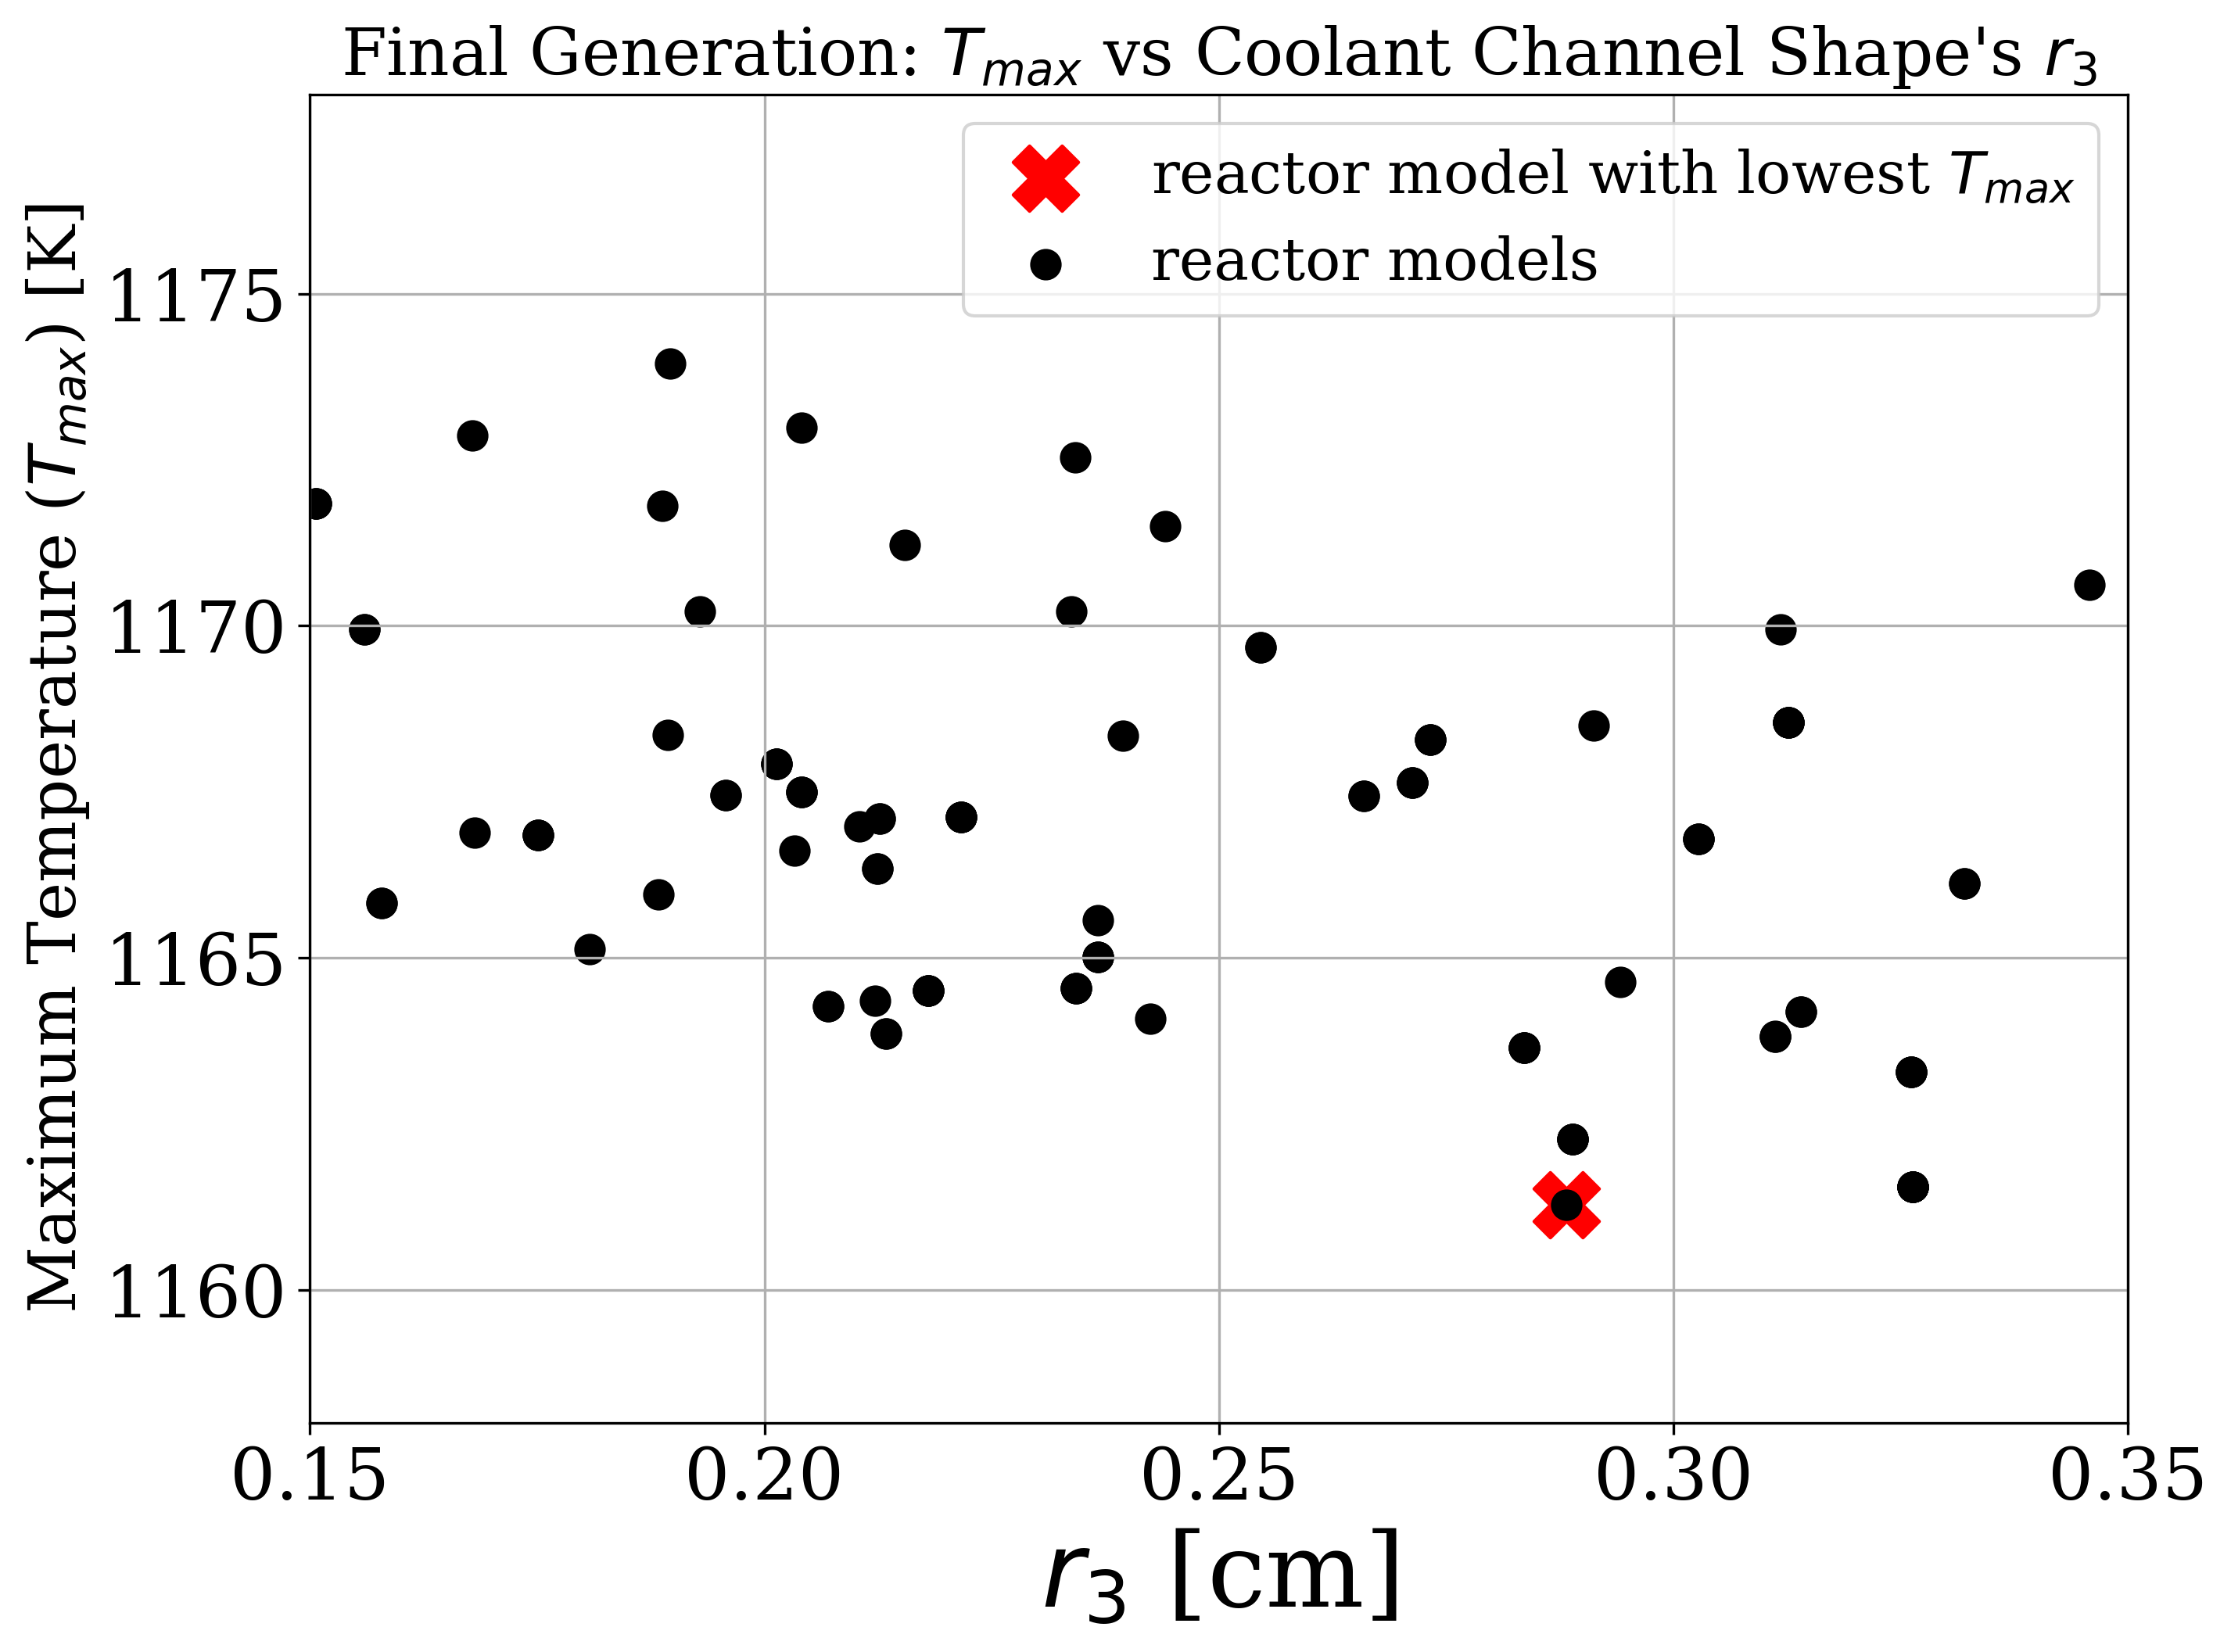
\includegraphics[width=\linewidth]{figures/a-1e-r3-pres.png}
            \caption{Plot of $T_{max}$ against $r_3$.}
            \label{fig:a-1e-r3} 
        \end{subfigure}
        \begin{subfigure}{0.3\textwidth}
            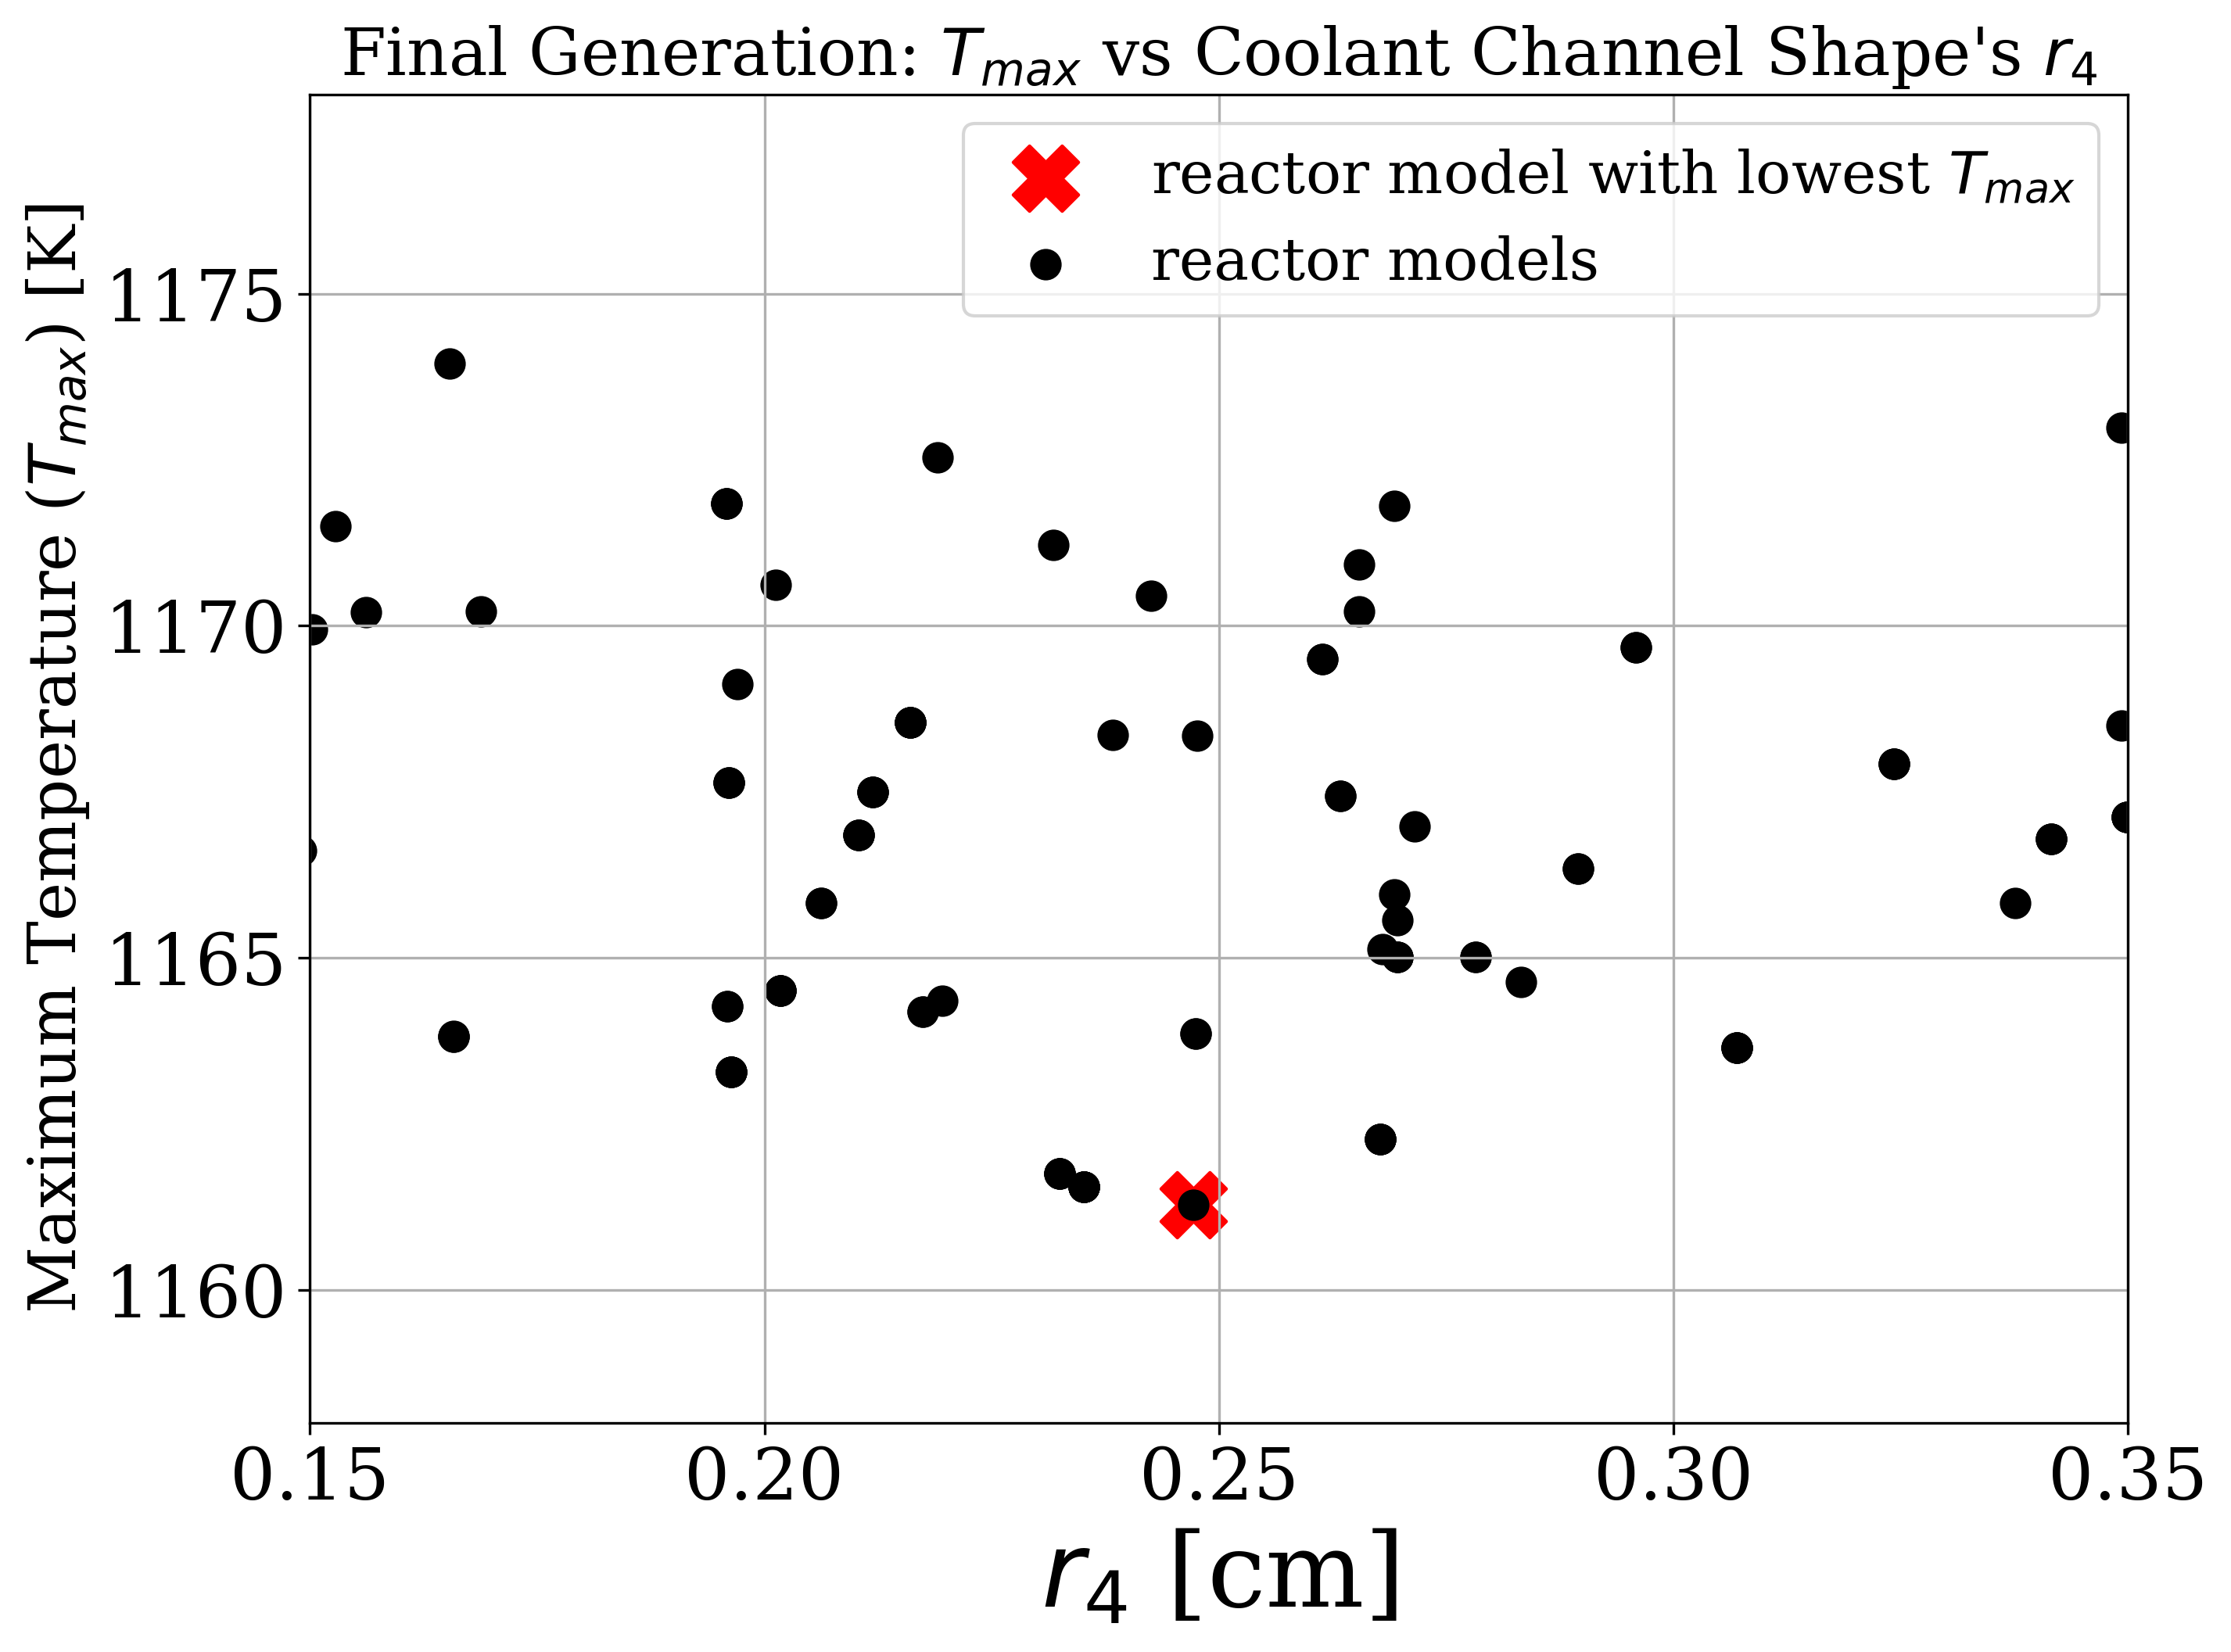
\includegraphics[width=\linewidth]{figures/a-1e-r4-pres.png}
            \caption{Plot of $T_{max}$ against $r_4$.}
            \label{fig:a-1e-r4} 
        \end{subfigure}
        \begin{subfigure}{0.3\textwidth}
            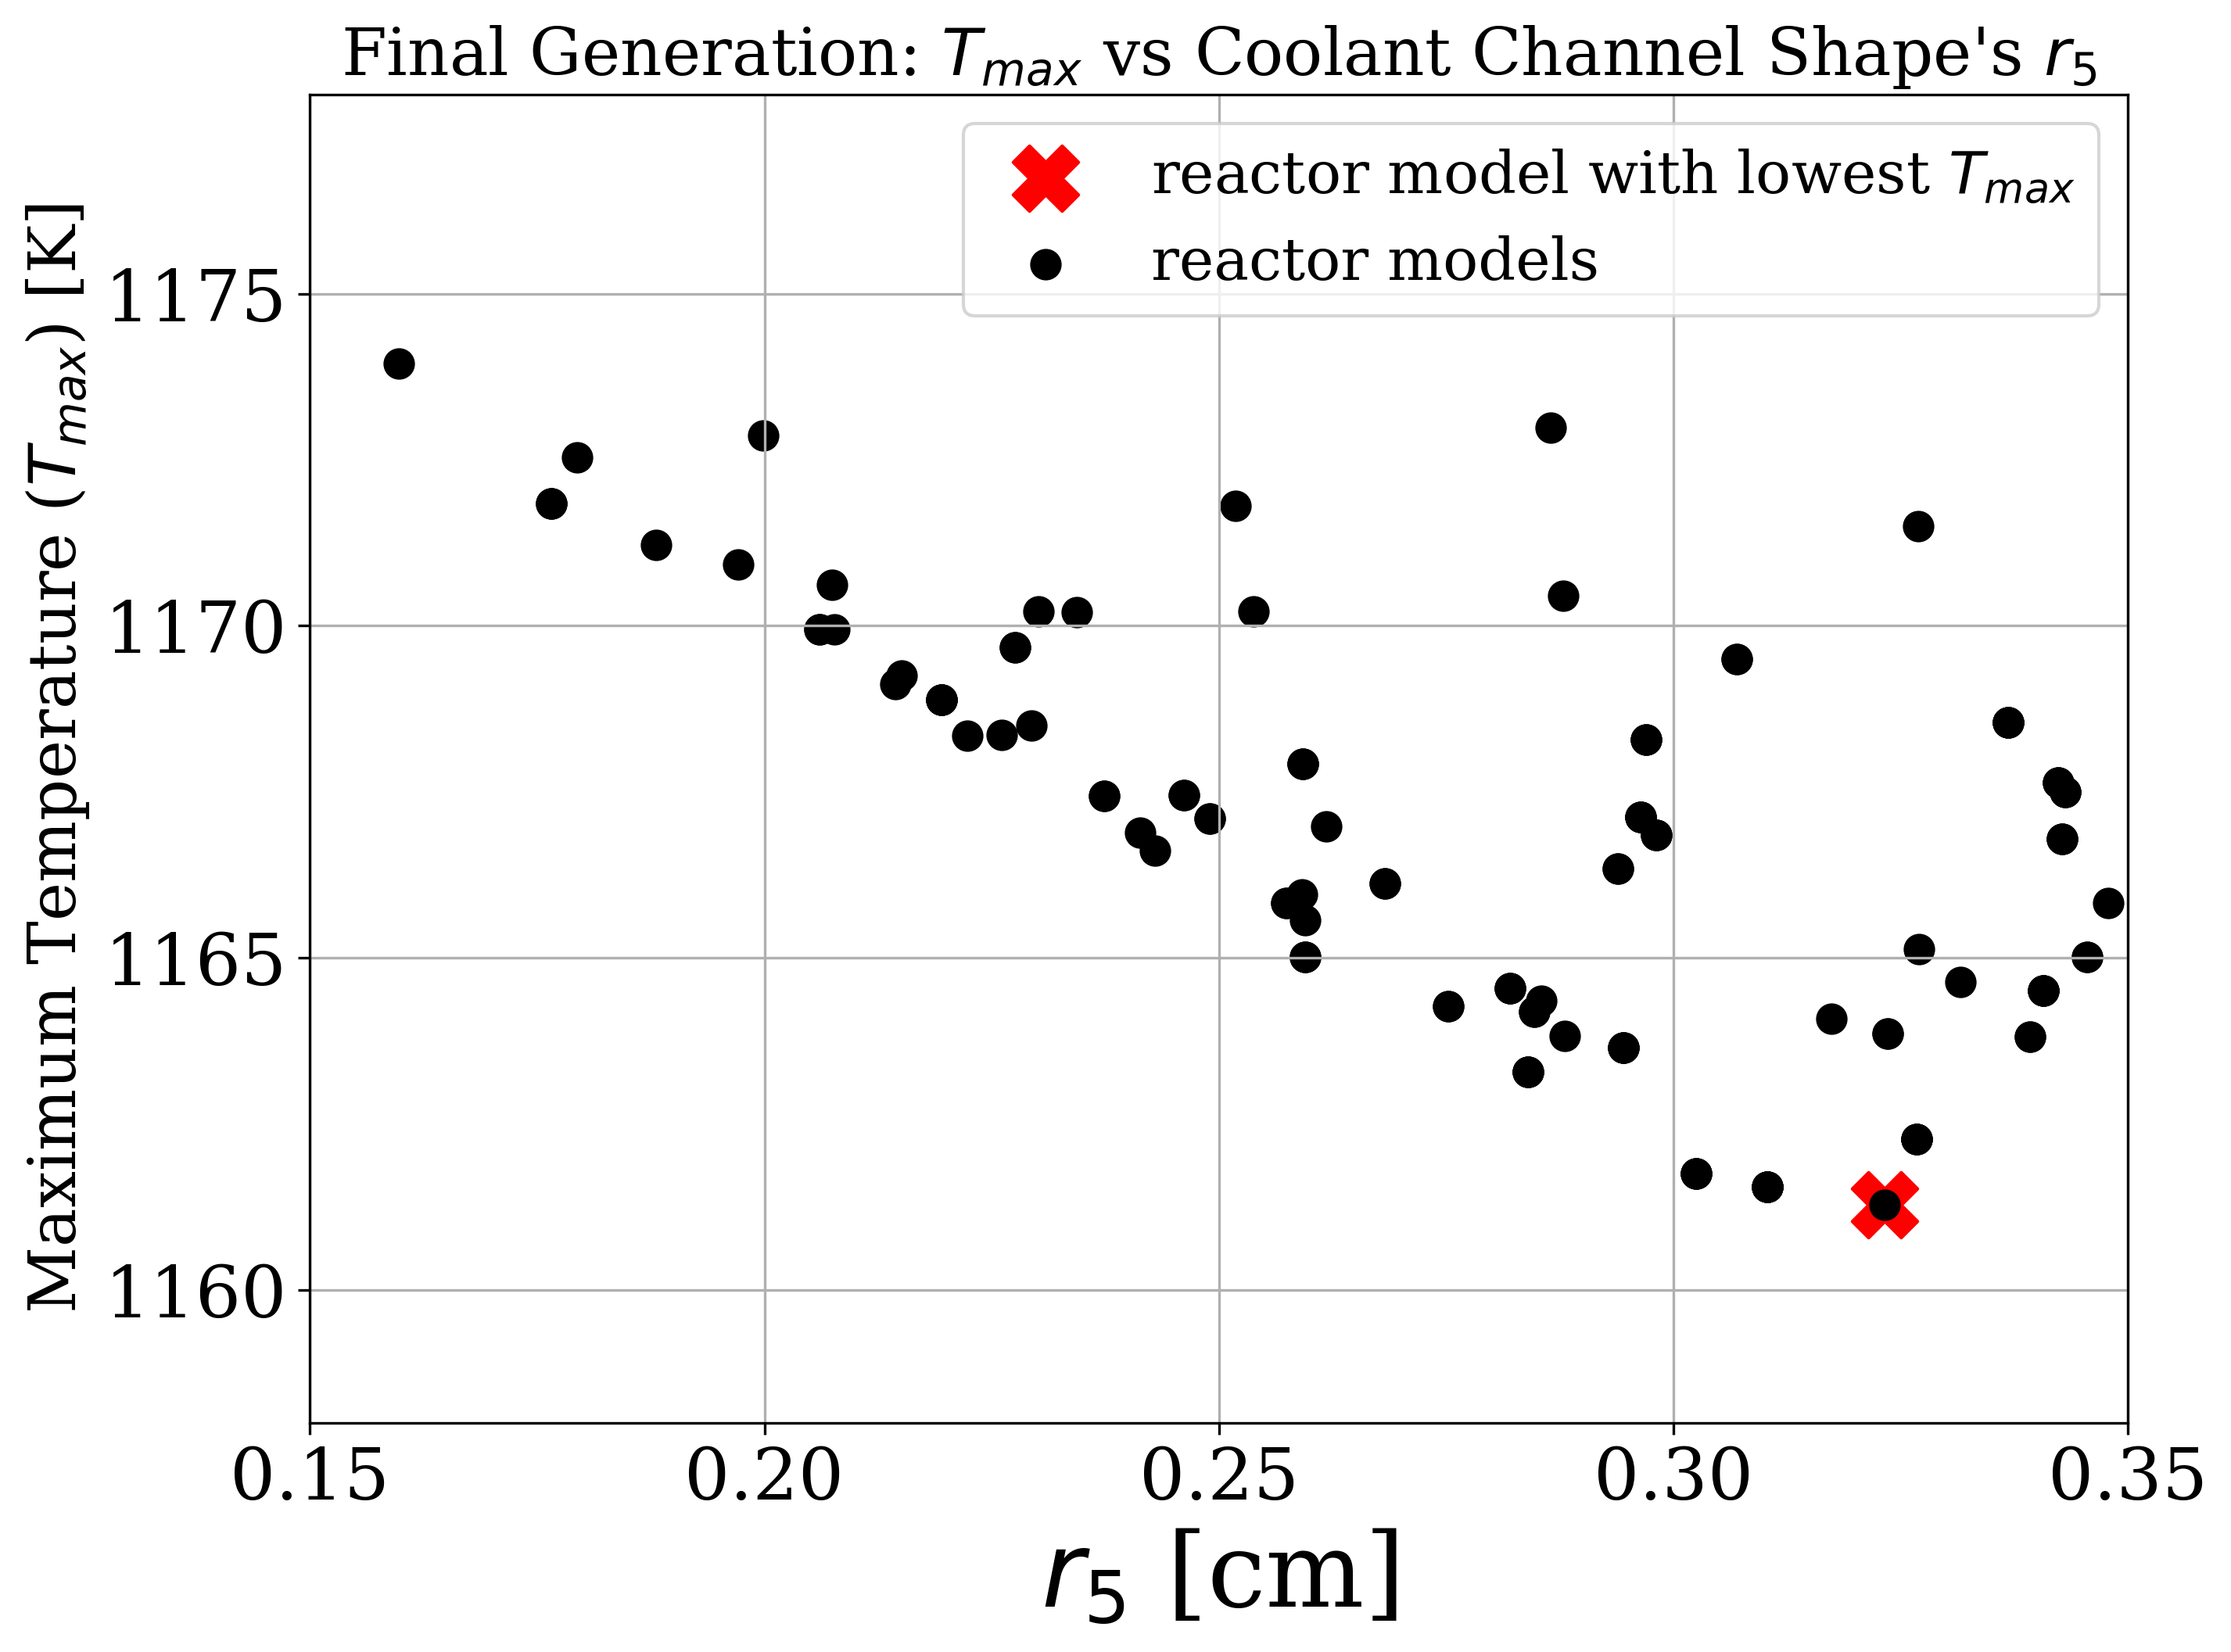
\includegraphics[width=\linewidth]{figures/a-1e-r5-pres.png}
            \caption{Plot of $T_{max}$ against $r_5$.}
            \label{fig:a-1e-r5} 
        \end{subfigure}
        \vspace{-0.3cm}
        \caption{Simulation a-1e's $T_{max}$ vs coolant channel shapes.}
    \end{figure}
\end{frame}

\begin{frame}
    \frametitle{AHTR One-Third Assembly Simulation a-1e Results}
    \begin{figure}
        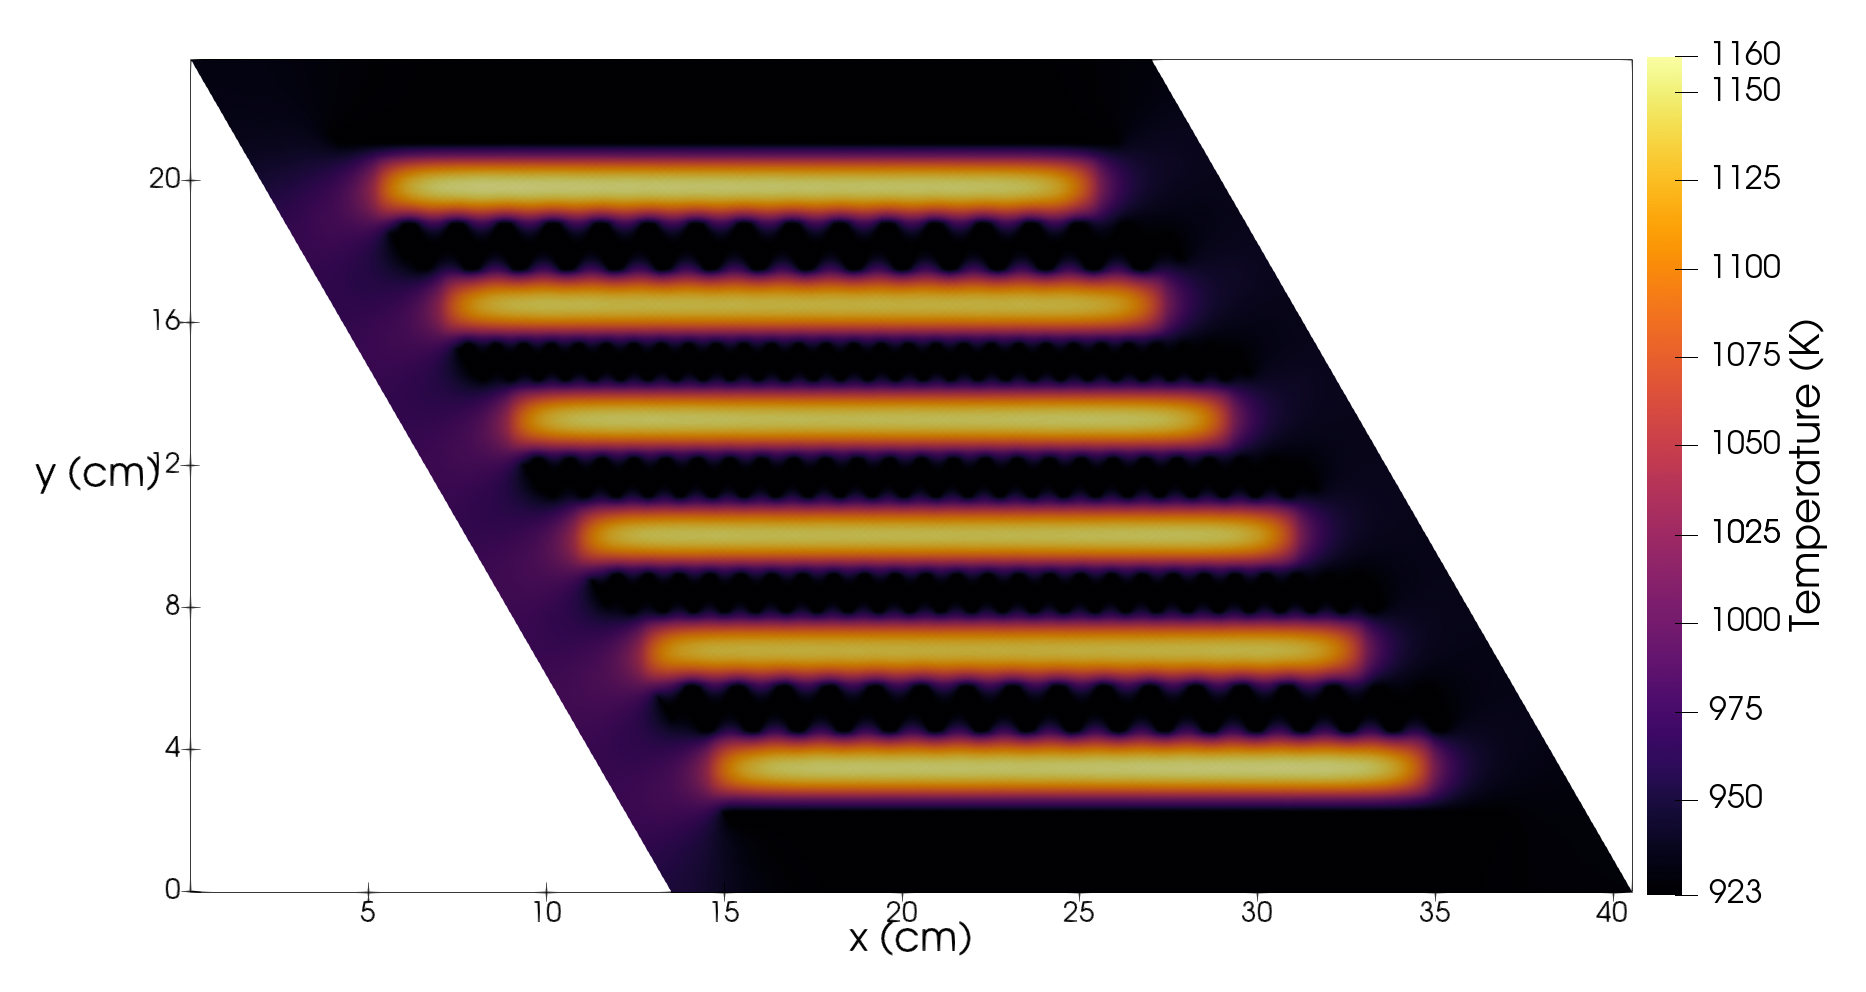
\includegraphics[width=0.55\linewidth]{../docs/figures/a-1e-temp-distribution-2d.png} 
        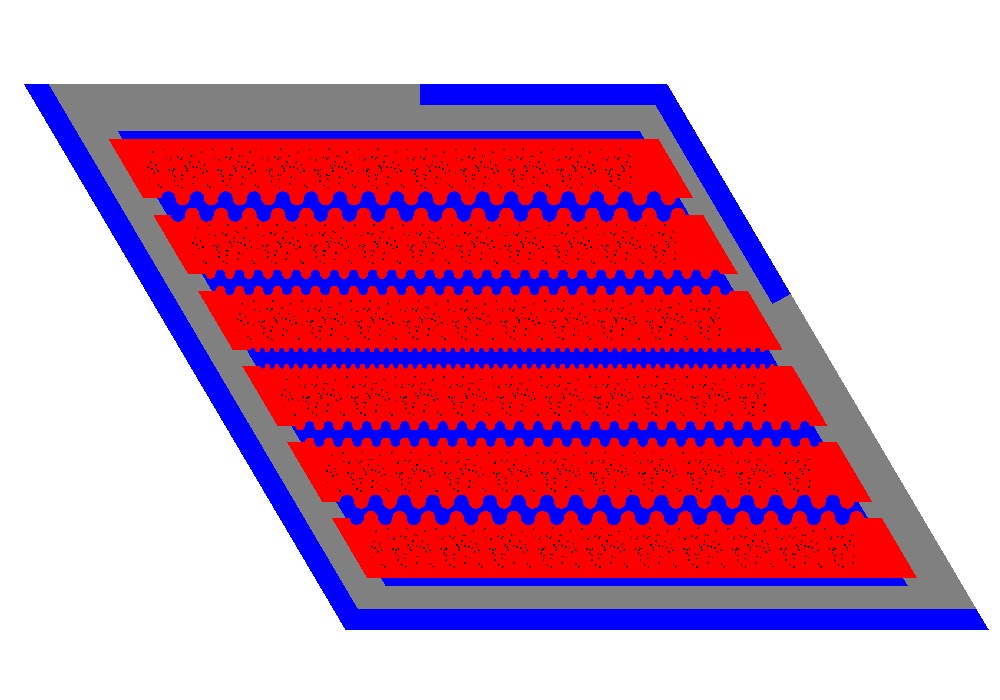
\includegraphics[width=0.4\linewidth]{../docs/figures/coolant-channel-shape-assem.png} 
        \caption{Temperature Distribution in simulation a-1e's most-minimized $T_{max}$ reactor 
        model.}
    \end{figure}
    \begin{tcolorbox}[colback=illiniorange,colframe=illiniorange!50!black]
    \textbf{FLiBe channels located closest to temperature peaks shows a \\ negative 
    correlation with $T_{max}$.}
    \end{tcolorbox}
\end{frame}

\begin{frame}
    \frametitle{Single-Objective Optimization Major Takeaways}
    \textbf{Minimize $PF_{total}$ Objective} 
    \begin{itemize}
        \item Driven by maximizing total fission reaction rate
        \item Influences oscillations in TRISO's spatial distribution
        \item No correlation with coolant channel shape  
    \end{itemize}

    \vspace{0.2cm}
    \textbf{Minimize $T_{max}$ Objective}
    \begin{itemize}
        \item A flatter TRISO distribution minimizes $T_{max}$
        \item FLiBe channels located closest to temperature peaks shows a negative 
        correlation with $T_{max}$
    \end{itemize}

    \vspace{0.2cm}
    \textbf{Minimize $PPF_{fuel}$ Objective} 
    \begin{itemize}
        \item Driven by flattening thermal flux distribution
        \item Influences oscillations in TRISO's spatial distribution
        \item No correlation with coolant channel shape  
    \end{itemize}
\end{frame}

\begin{frame}
    \frametitle{AHTR One-Third Assembly Simulation a-2b Results}
    I vary $PF_{total}$ and \textbf{a, b, c, d, e f} ($\rho_{TRISO}(\vec{x}, \vec{y}$))
    to minimize $PF_{total}$ and $PPF_{fuel}$. 

    \vspace{0.1cm}
    \begin{figure}
        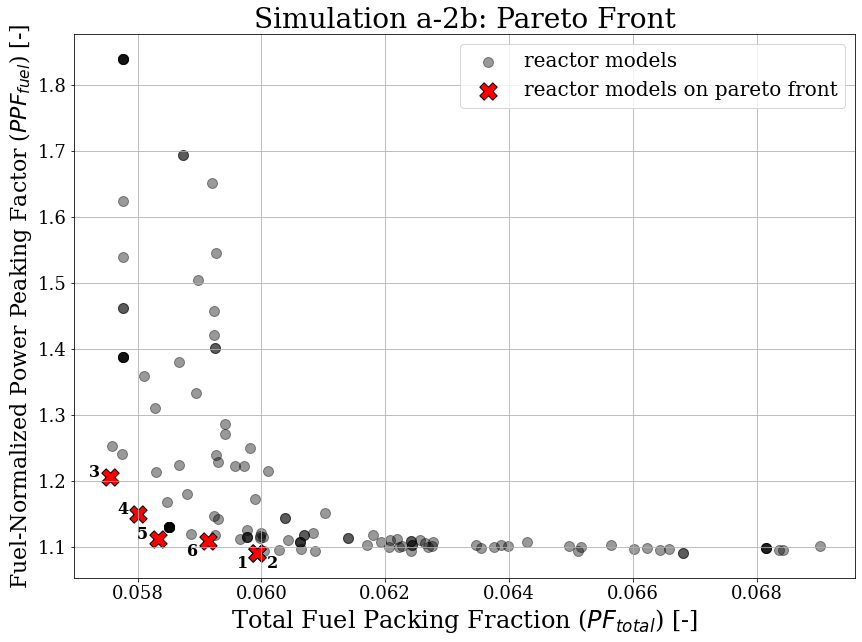
\includegraphics[width=0.73\linewidth]{../docs/figures/assem-obj-2-pfppf-pareto.png} 
        \caption{Simulation a-2b Pareto Front.}
    \end{figure}
\end{frame}

\begin{frame}
    \frametitle{AHTR One-Third Assembly Simulation a-2b Results}
    \begin{figure}
        \only<1>{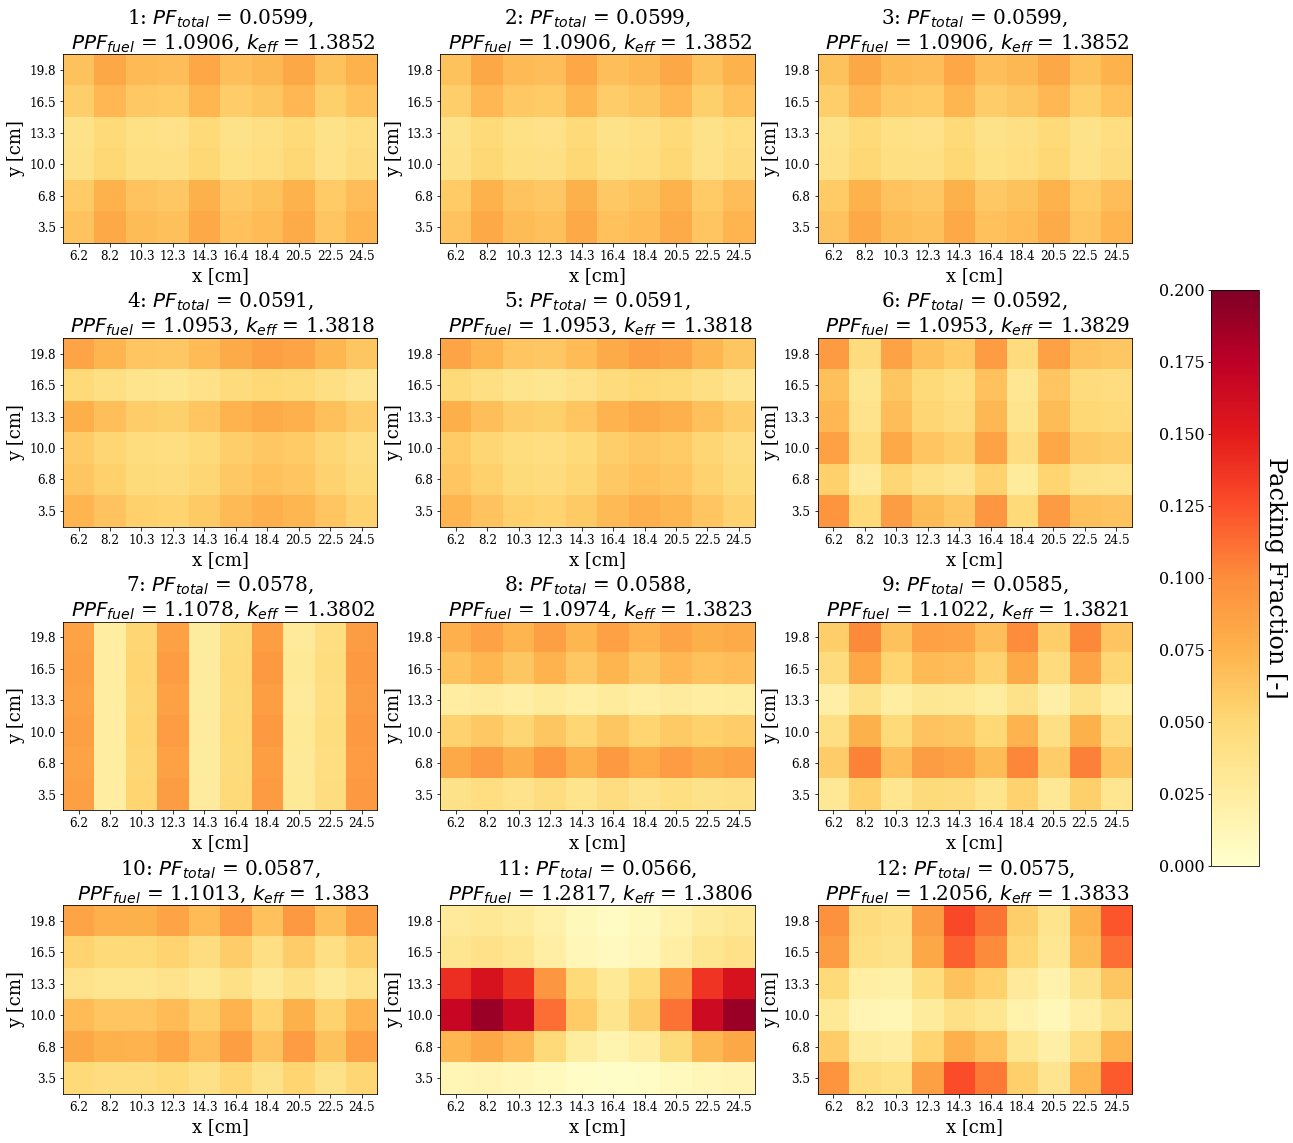
\includegraphics[width=0.9\linewidth]{../docs/figures/assem-obj-2-pfppf-pareto-distr.png}}
        \only<2>{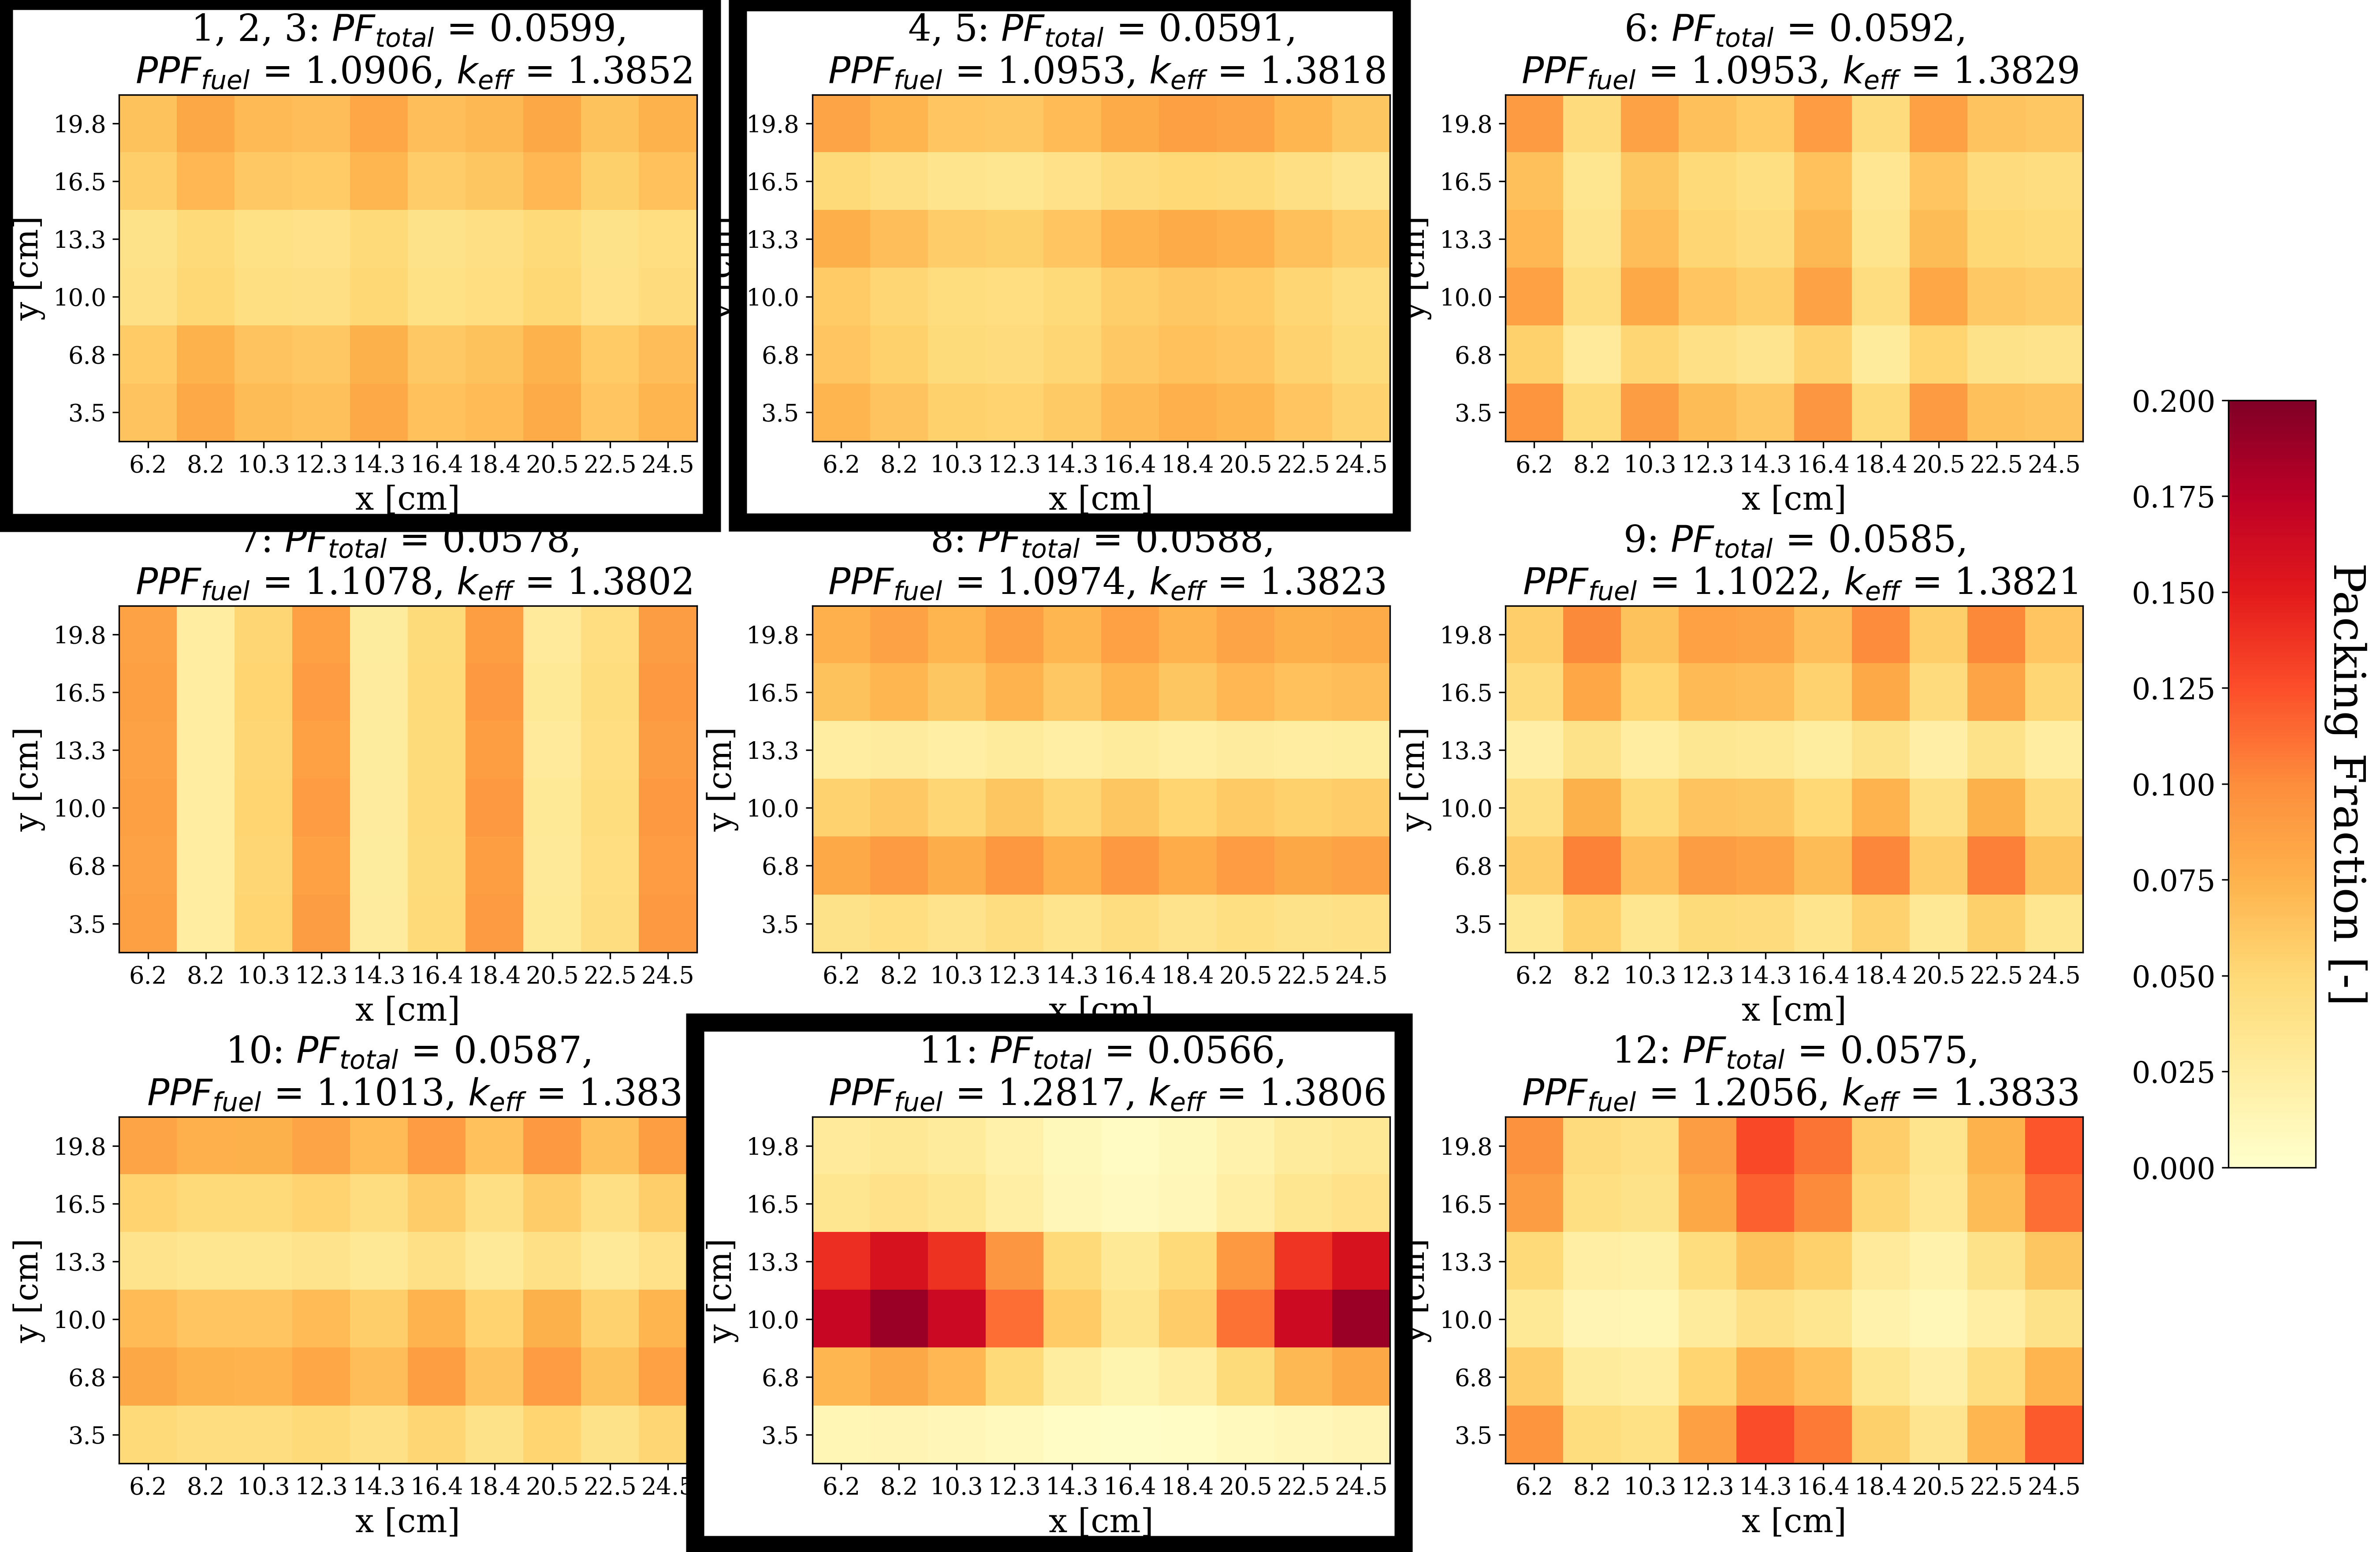
\includegraphics[width=0.9\linewidth]{figures/assem-obj-2-pfppf-pareto-distr-annotated.png}}
        \caption{Simulation a-2b Pareto Front's TRISO Distributions.}
    \end{figure}
\end{frame}

\begin{frame}
    \frametitle{AHTR One-Third Assembly Simulation a-2b Results}
    \vspace{-0.25cm}
    \begin{figure}
        \centering
        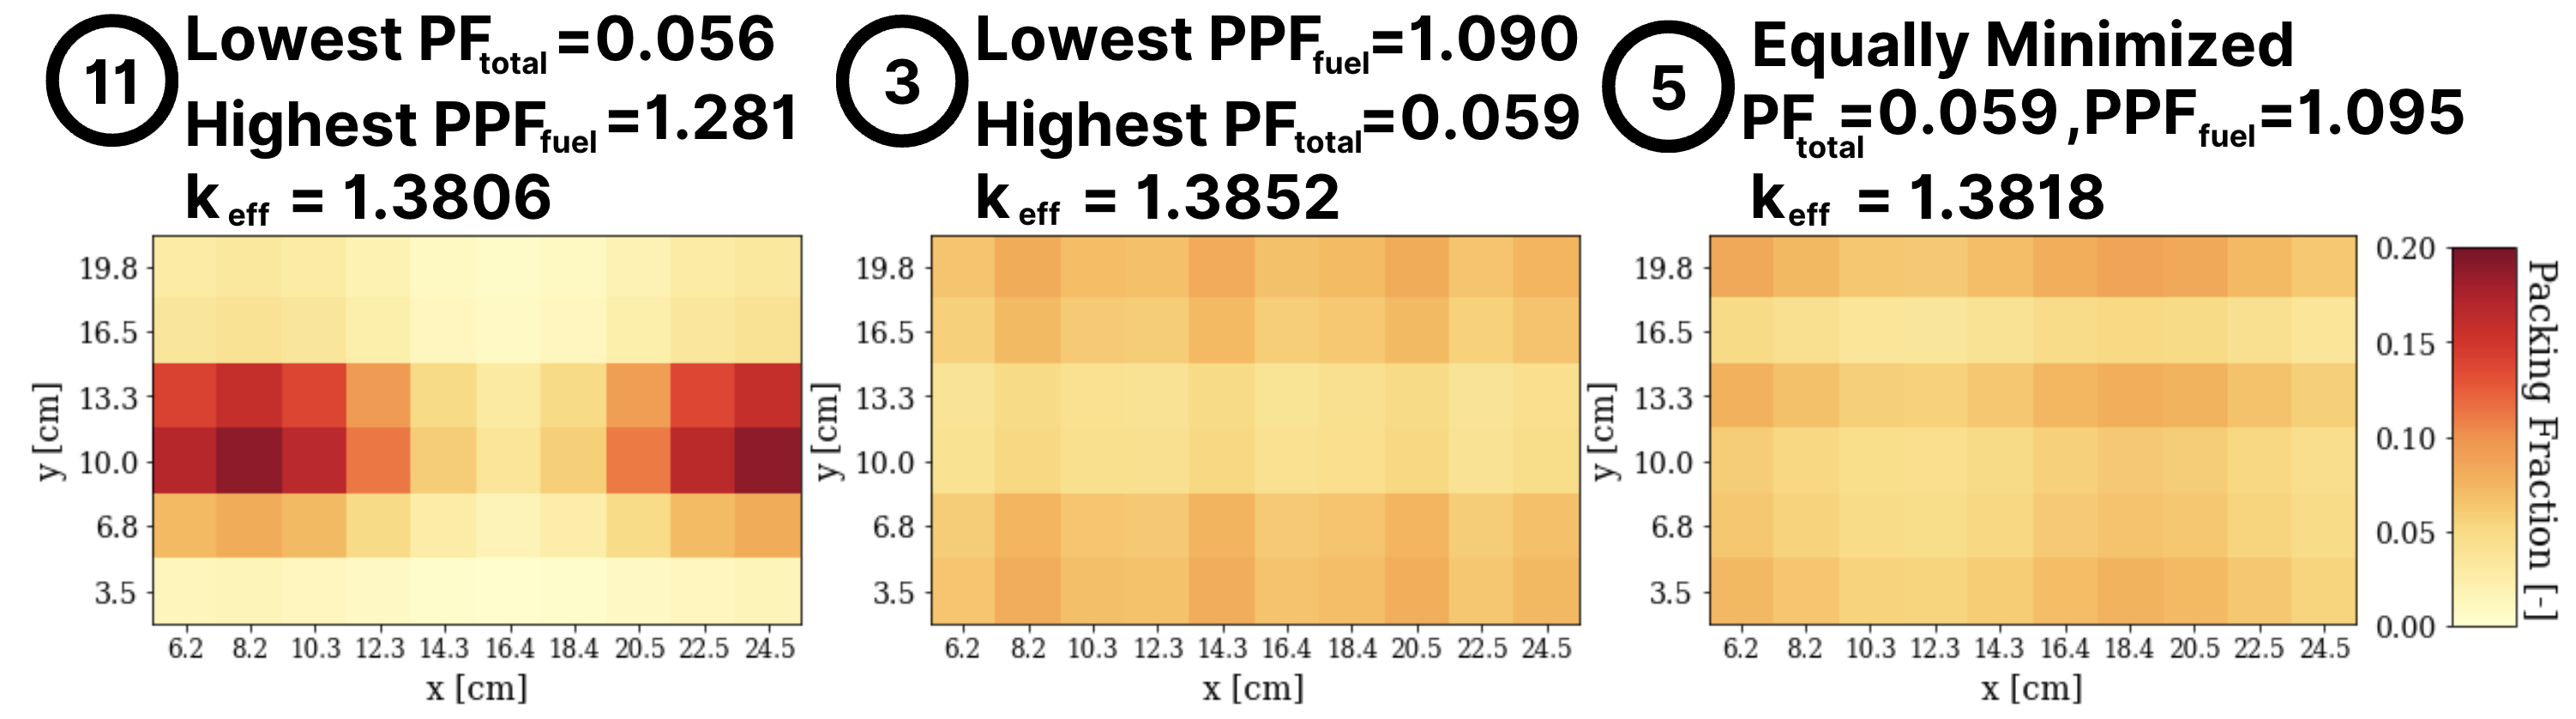
\includegraphics[width=\linewidth]{figures/a-2b-comparison-reactors.png}
    \end{figure}
    \vspace{-0.4cm}
    \begin{columns}
        \begin{column}{0.4\linewidth}
            \begin{figure}
                \centering
                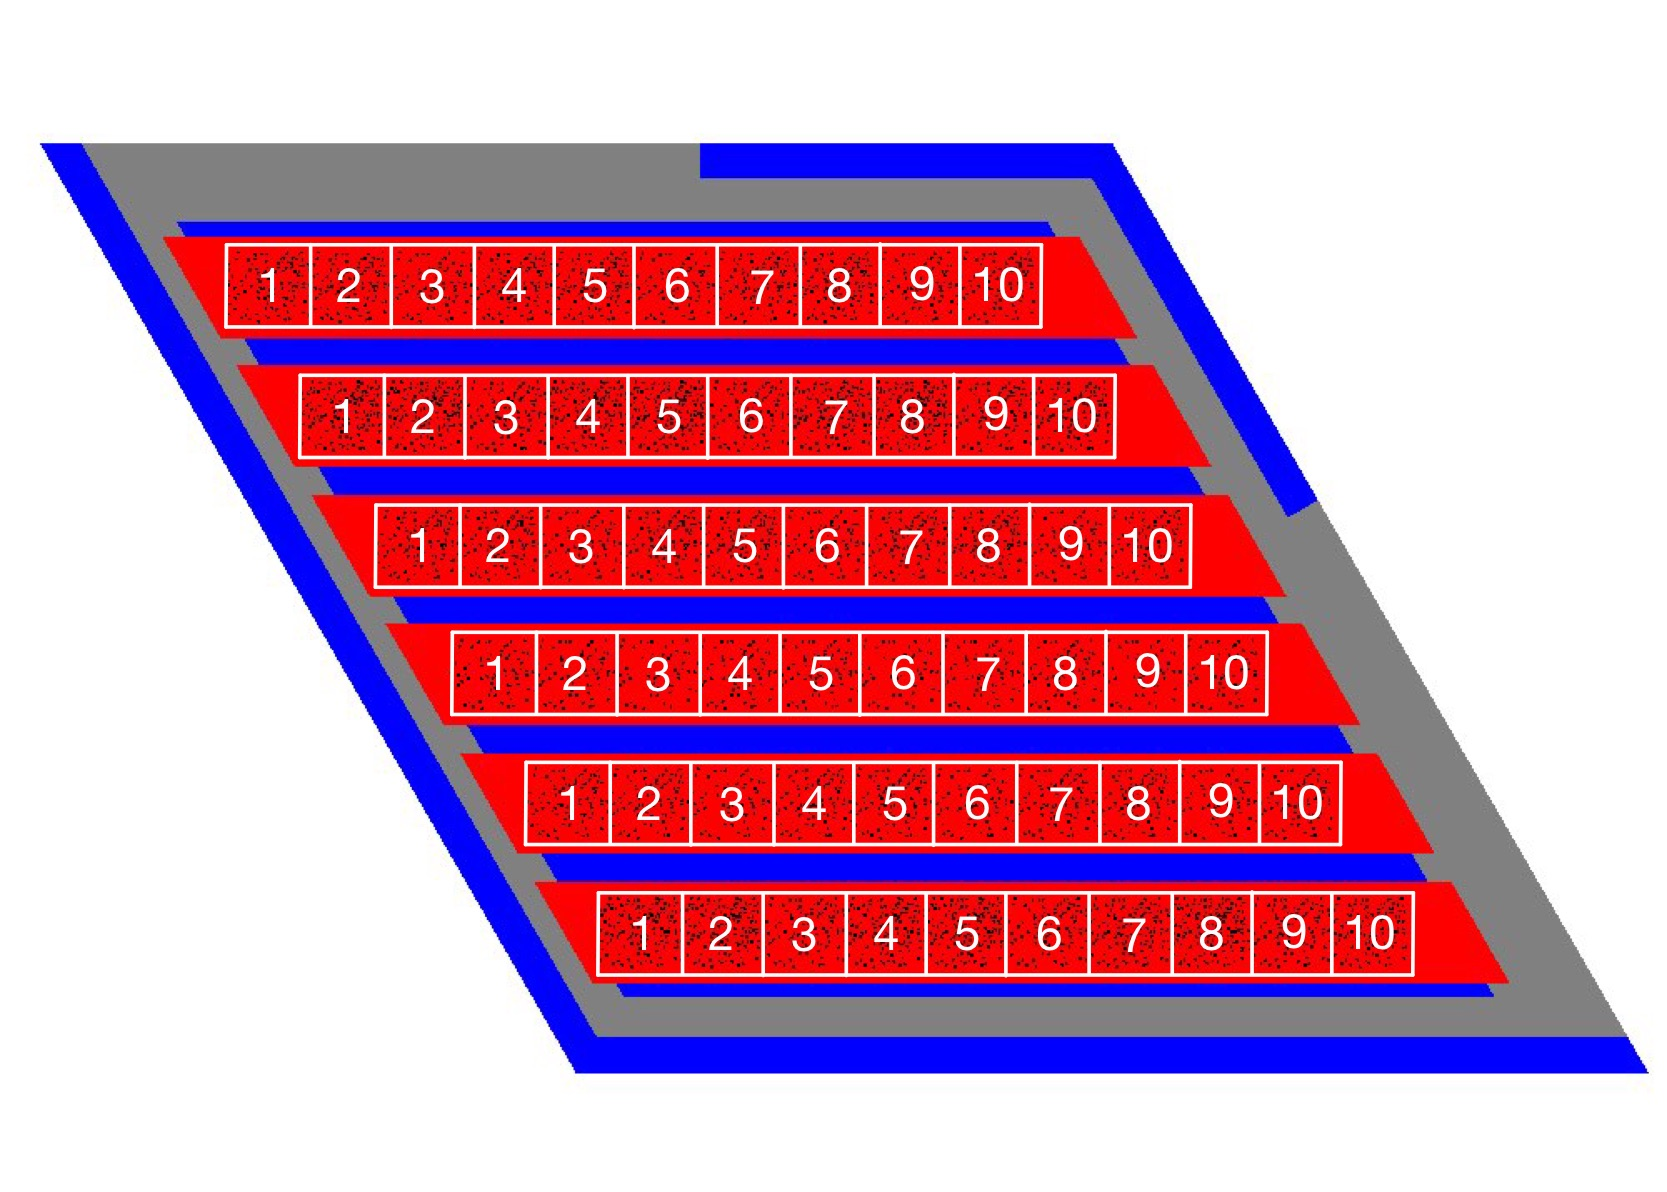
\includegraphics[width=\linewidth]{../docs/figures/ahtr_assembly.png} 
            \end{figure}
        \end{column}
        \begin{column}{0.6\linewidth}
            \small
            Minimize $PF_{total}$ is driven by \textbf{maximizing total fission 
            reaction rate} 
            \begin{itemize}
                \item Highest to lowest total fission reaction rate: reactor model 
                $1 \rightarrow 11 \rightarrow 5$
            \end{itemize}
            Minimize $PPF_{fuel}$ objective is driven by \textbf{flattening thermal 
            flux distribution} 
            \begin{itemize}
                \item Most to least flat thermal flux: reactor model 
                $1 \rightarrow 5 \rightarrow 11$
            \end{itemize}
        \end{column}
    \end{columns}
    \begin{tcolorbox}[colback=illiniorange,colframe=illiniorange!50!black]
        Minimize $PF_{total}$ and Minimize $PPF_{fuel}$ objectives 
        influence each other resulting in \textbf{unexpected TRISO distributions at 
        different $PF_{total}$ values}. 
    \end{tcolorbox}
\end{frame}

\begin{frame}
    \frametitle{AHTR One-Third Assembly Simulation a-3b Results}
    \begin{columns}
    \begin{column}{0.35\textwidth}
        \begin{block}{Simulation a-3b}
            \begin{itemize}
            \item Vary $PF_{total}$, \textbf{a, b, c, d, e f} ($\rho_{TRISO}(\vec{x}, 
            \vec{y}$)), and $r_1, r_2, r_3, r_4, r_5$ (coolant channel shape) 
            \item Minimize all three objectives: $PF_{total}$, $T_{max}$ and $PPF_{fuel}$.
            \item 6 generations 
            \item 128 reactor models per gen 
            \item Total runtime: 1528 Theta node-hours 
            \end{itemize}
            \end{block}
        \end{column}
    \begin{column}{0.7\textwidth}
    \begin{figure}
        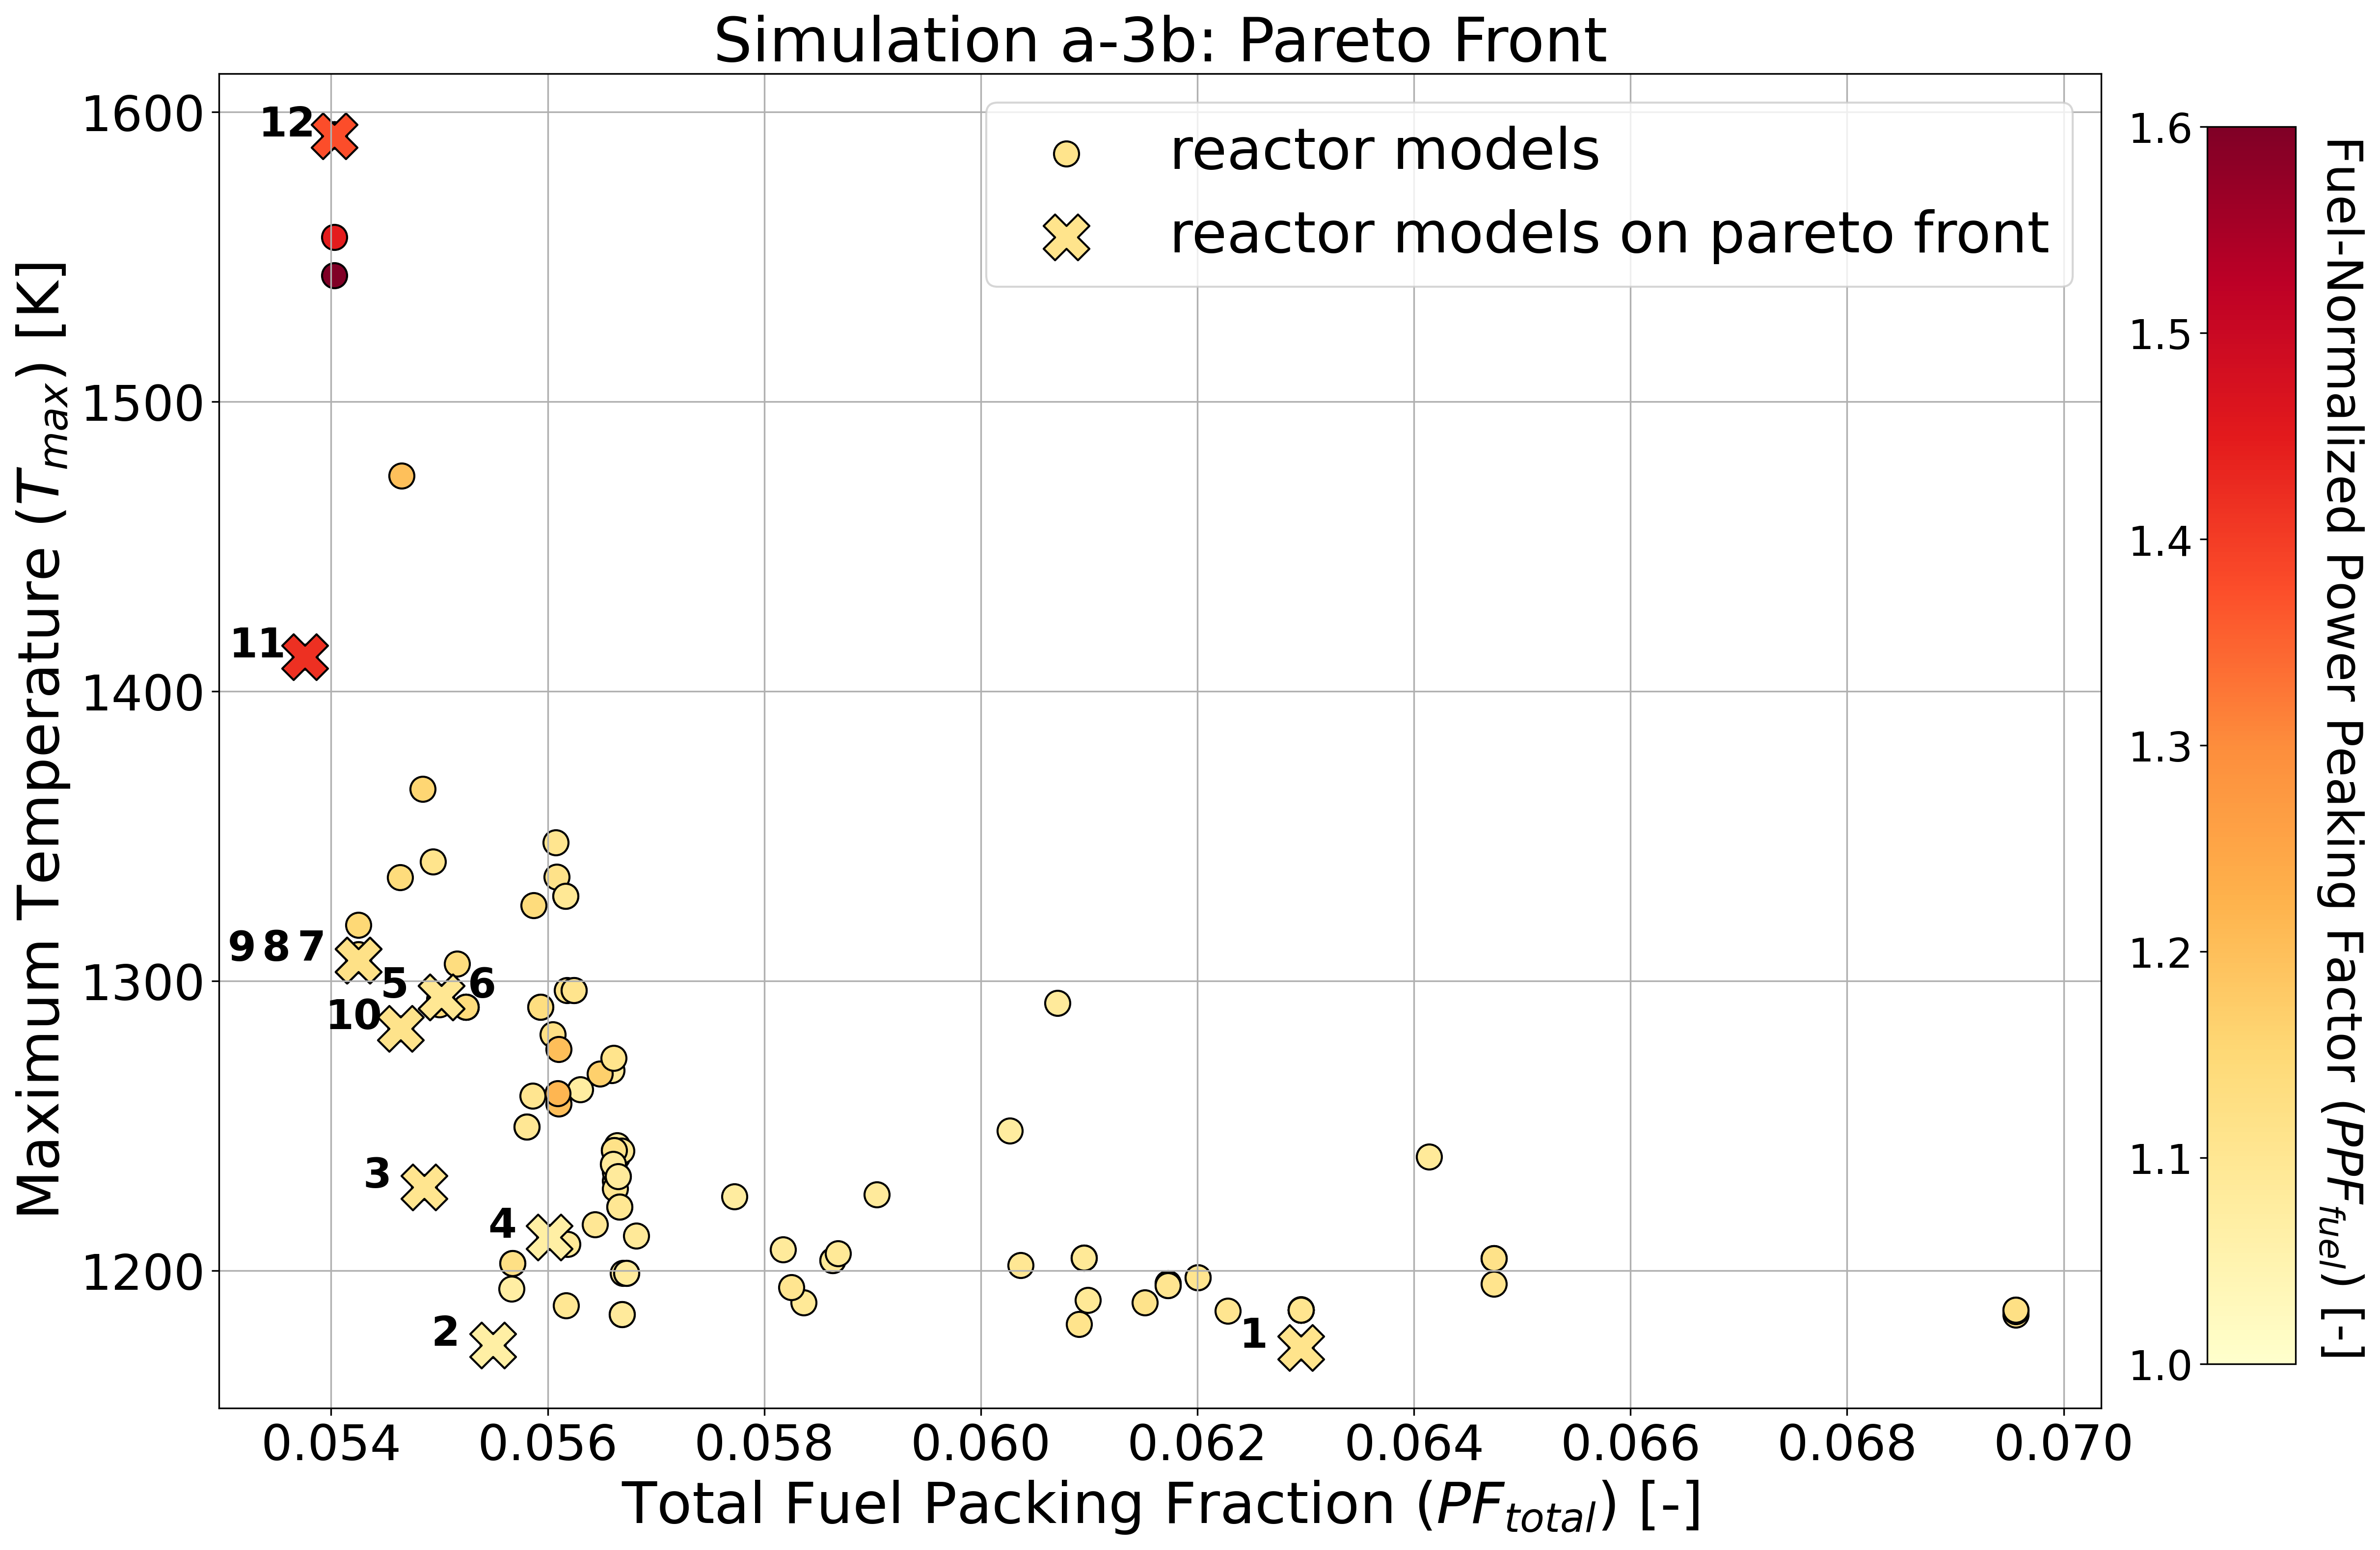
\includegraphics[width=\linewidth]{../docs/figures/assem-obj-3-all-2d.png} 
        \caption{Plot of final generation's reactor models' 
        $PF_{total}$ against $T_{max}$ against $PPF_{fuel}$ as a color dimension. 
        Crosses indicate the reactor models on the Pareto front.}
    \end{figure}
    \end{column}
\end{columns}
\end{frame}

\begin{frame}
    \frametitle{AHTR One-Third Assembly Simulation a-3b Results}
    \begin{figure}
        \only<1>{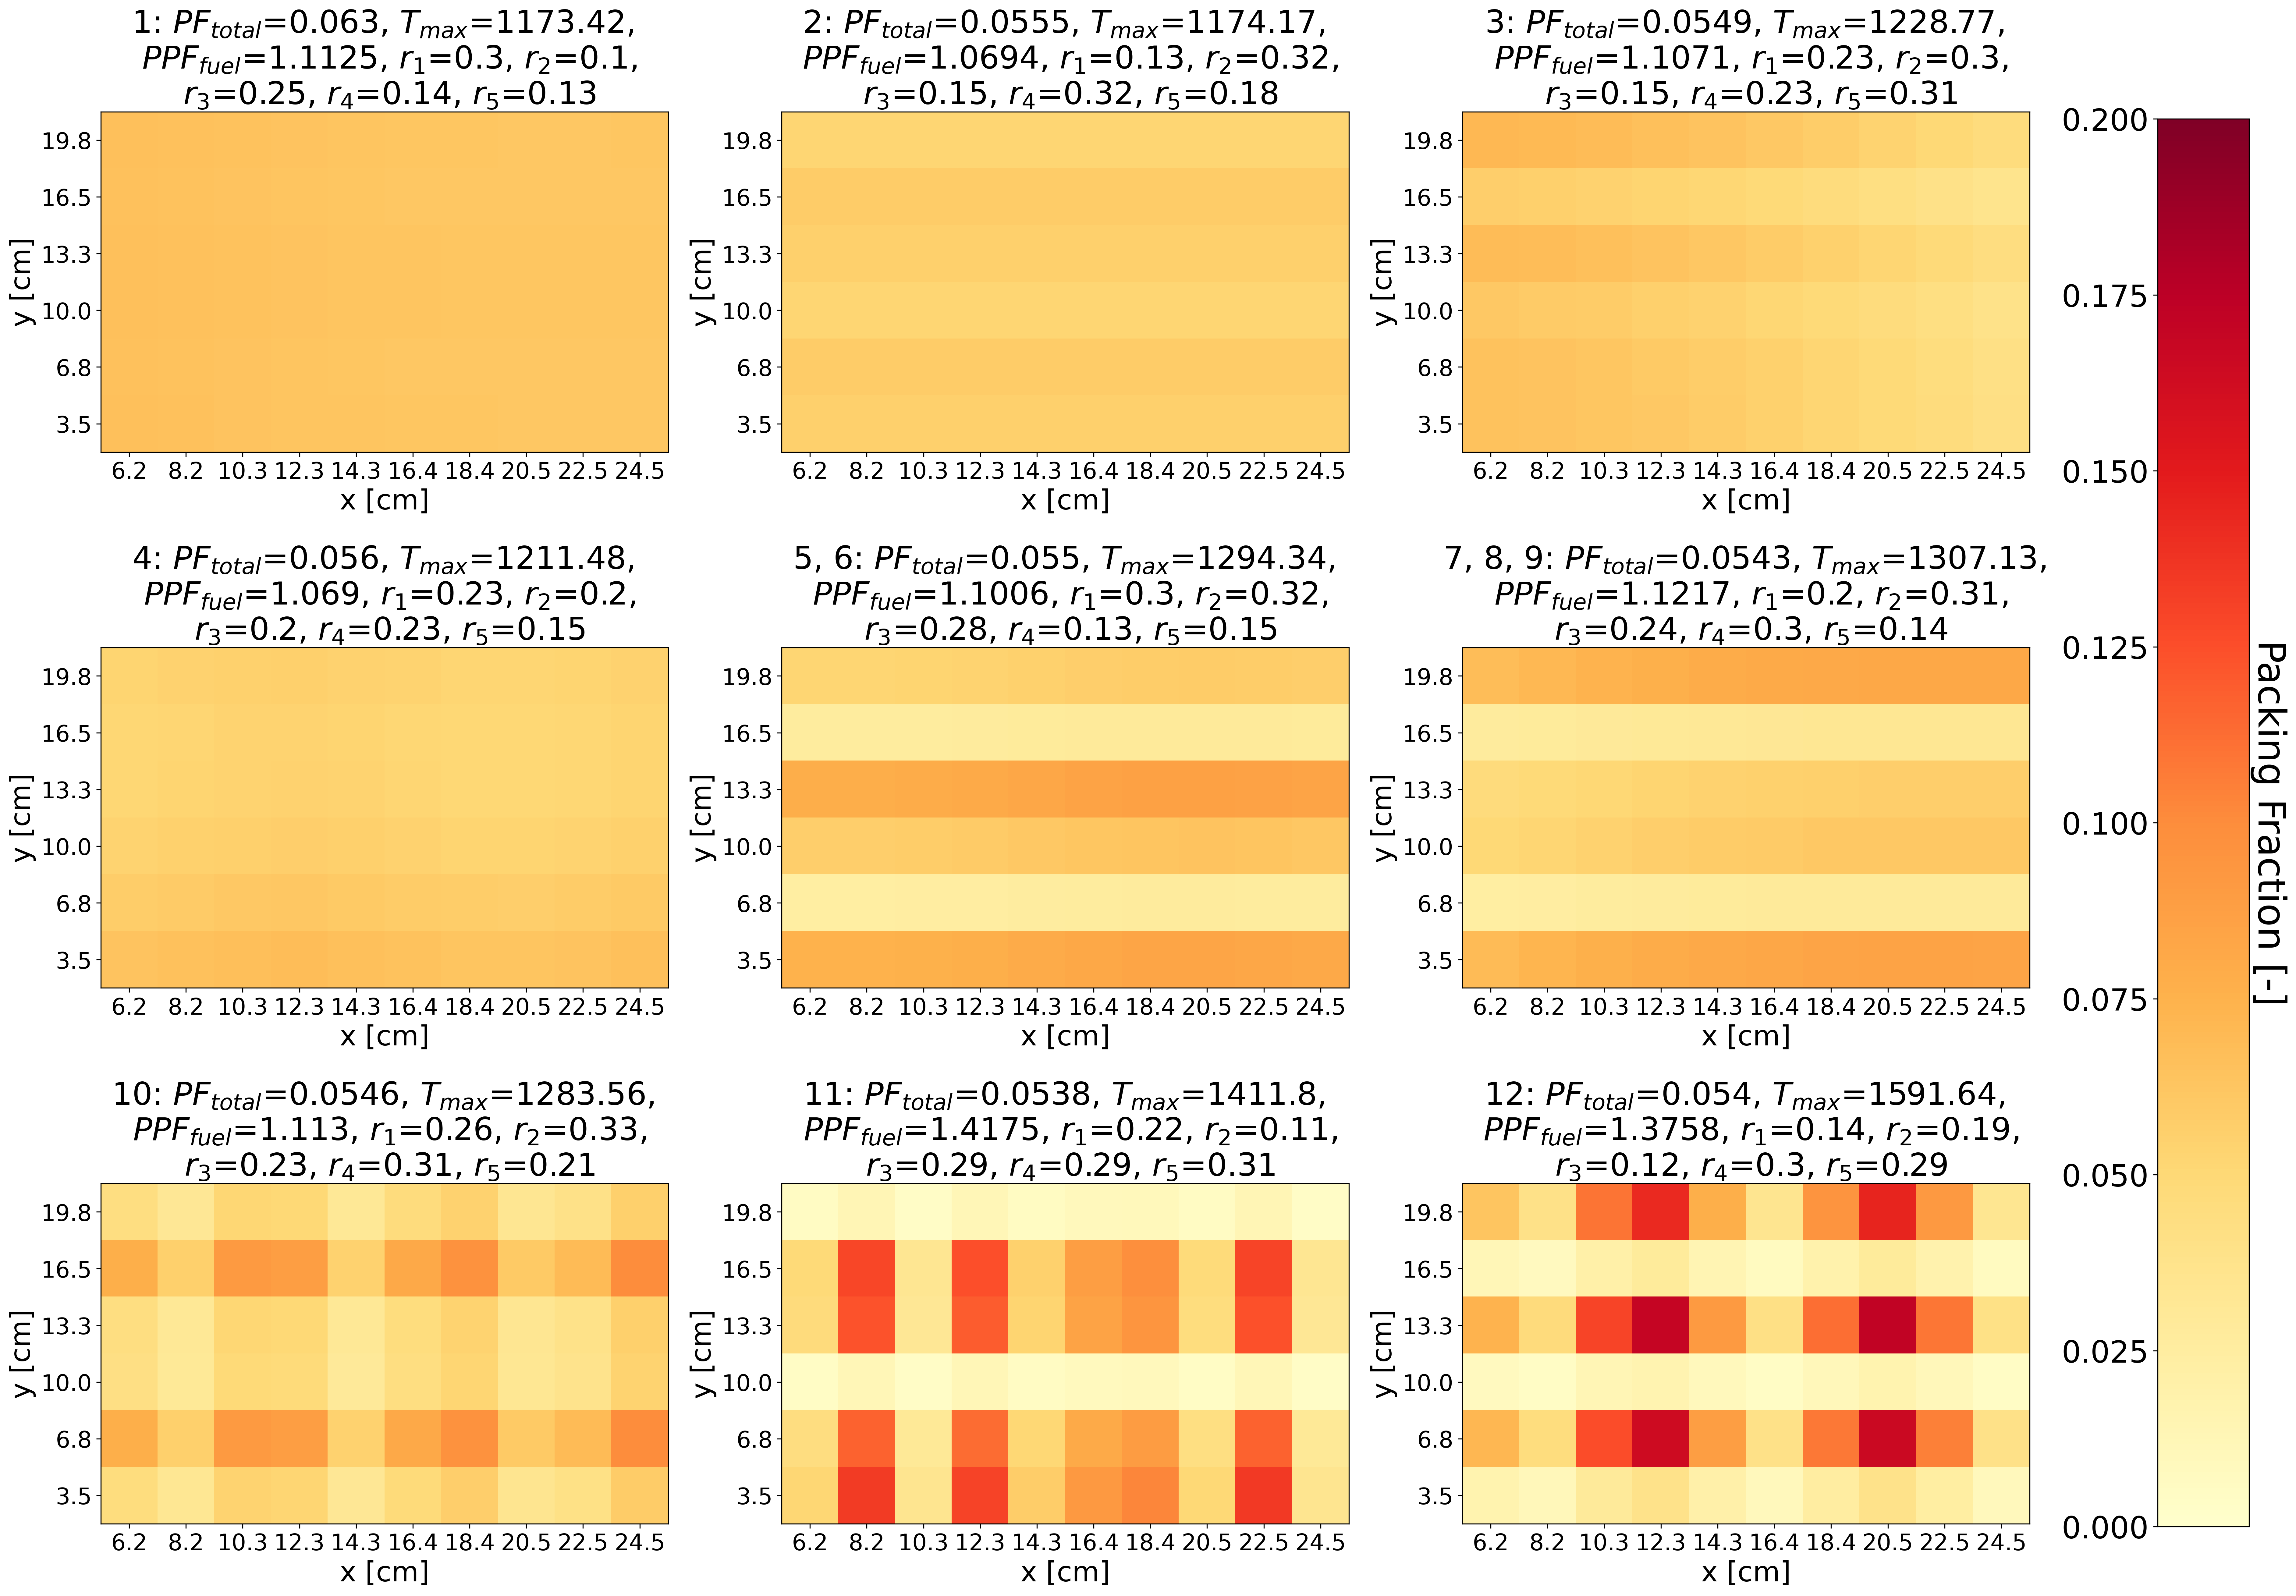
\includegraphics[width=0.8\linewidth]{../docs/figures/assem-obj-3-all-distr.png}}
        \only<2>{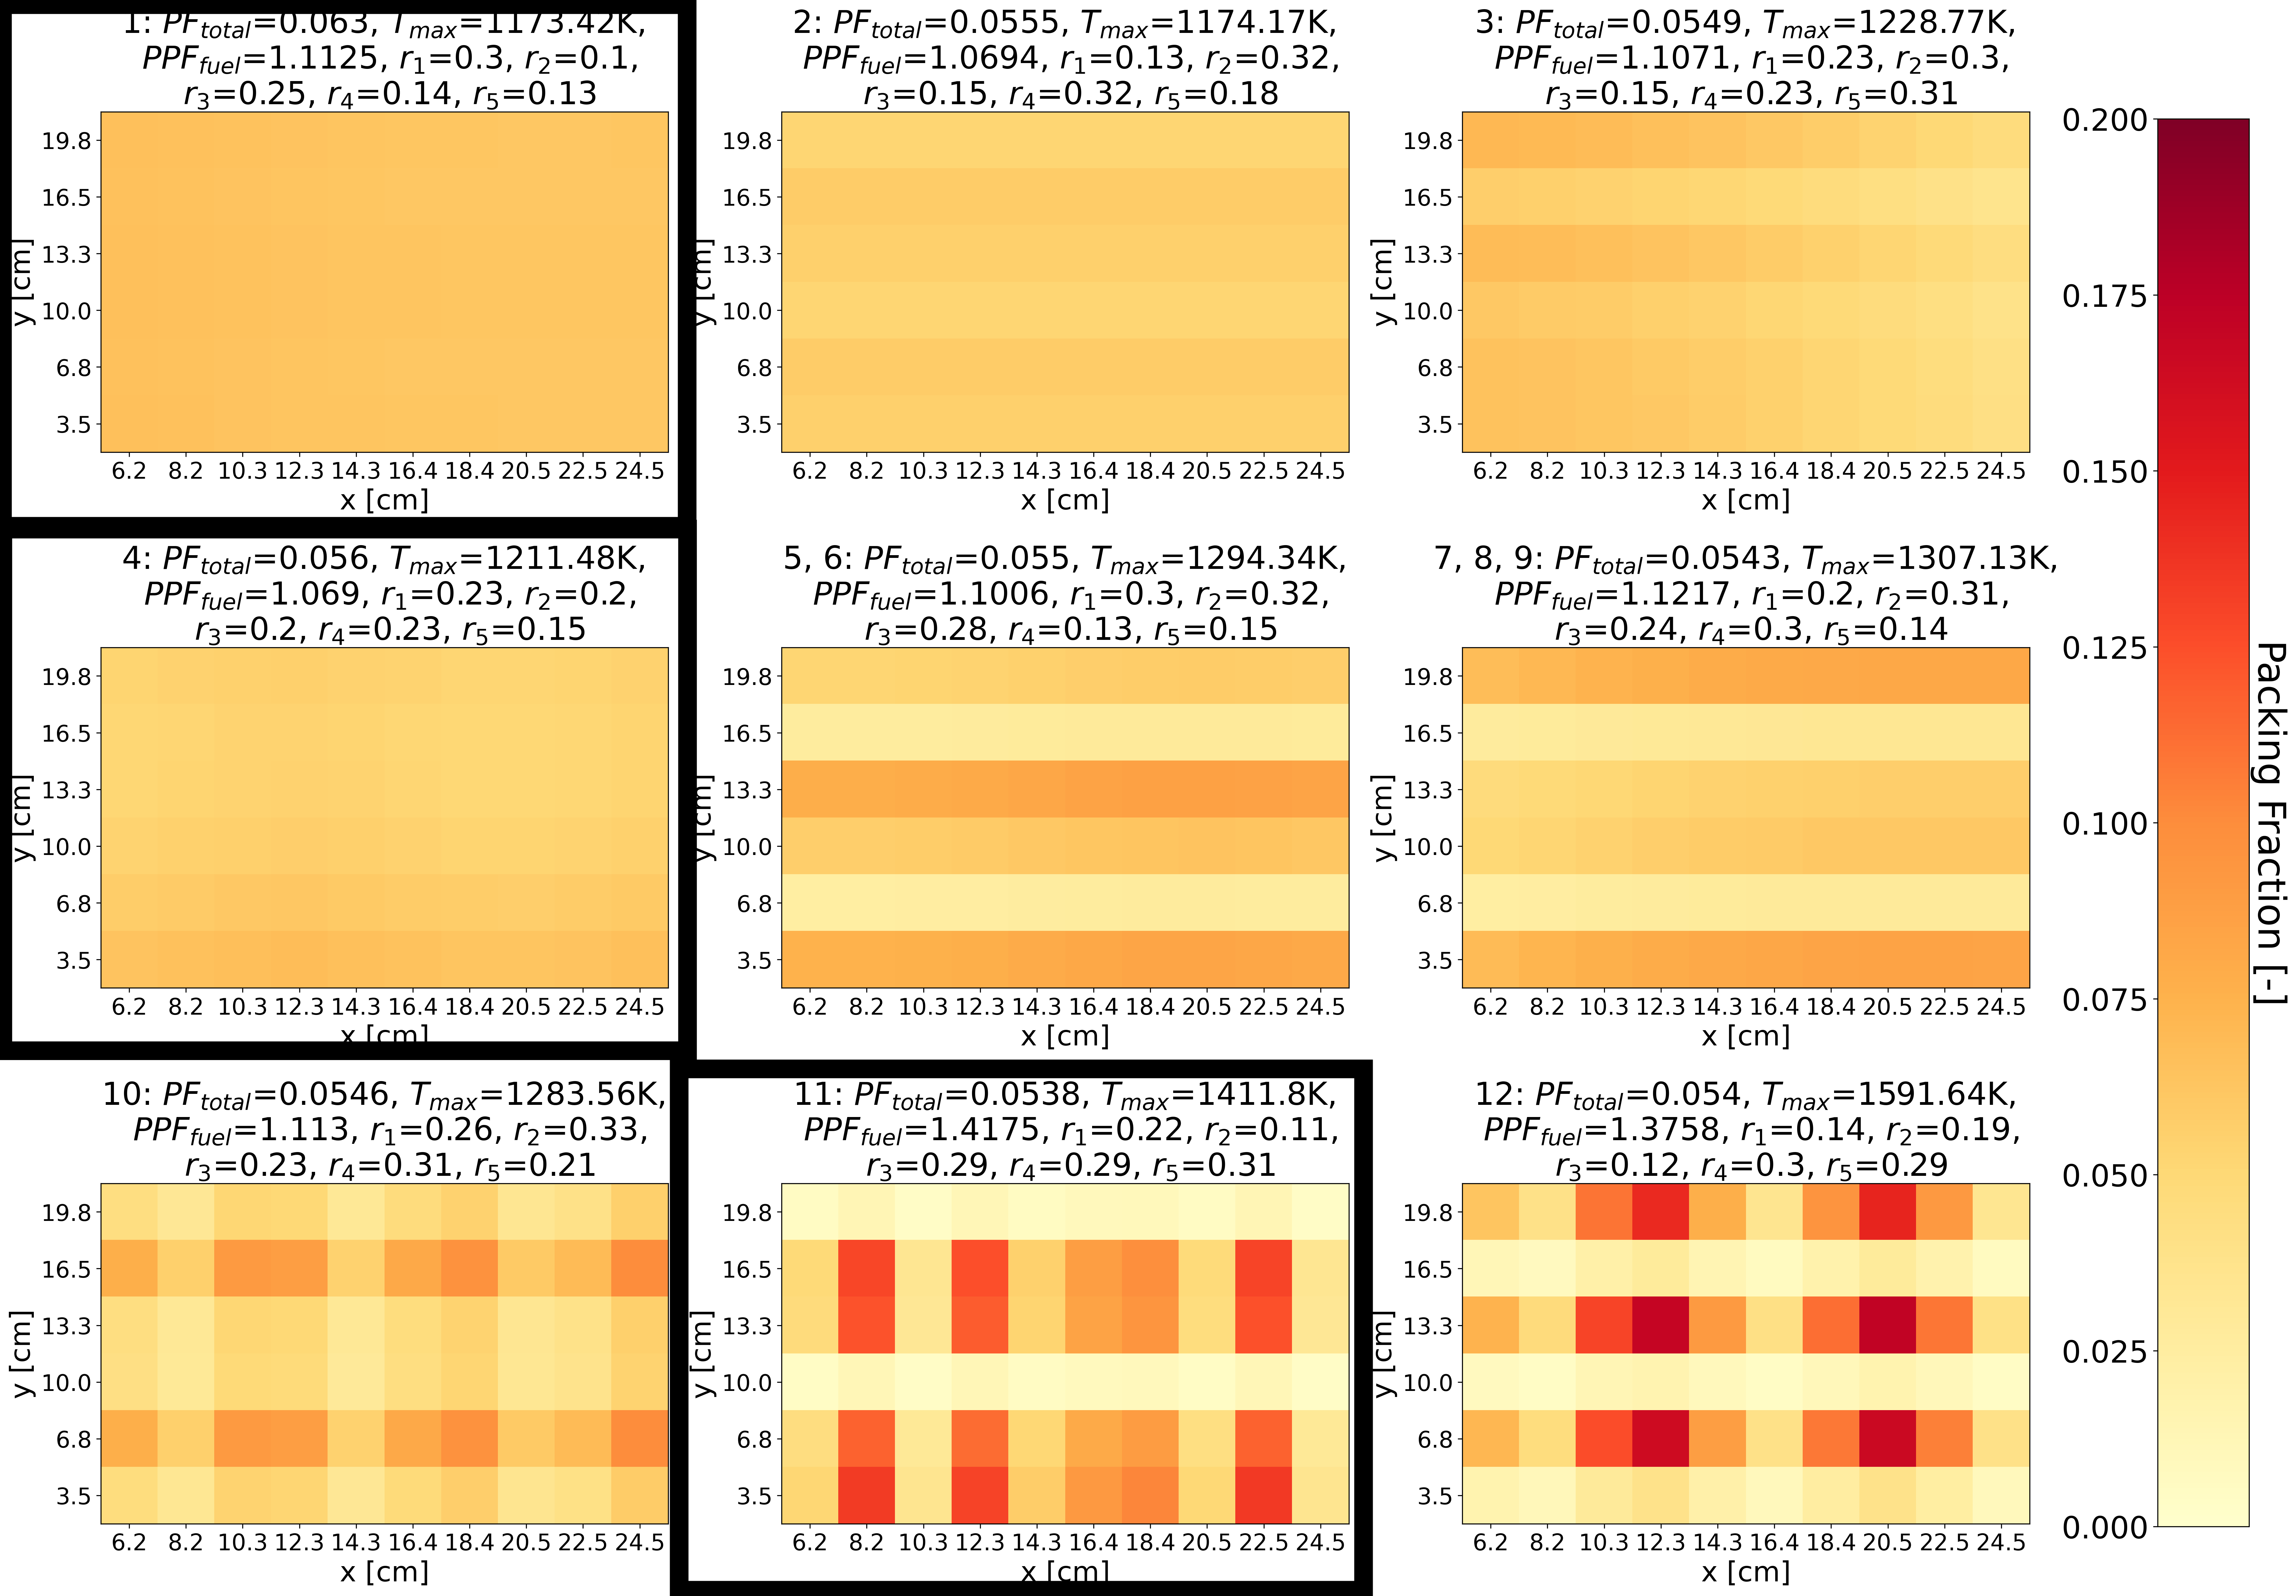
\includegraphics[width=0.8\linewidth]{figures/assem-obj-3-all-distr-annotated.png}}  
        \caption{TRISO distributions for the 12 reactor models on simulation 
        a-3b's Pareto front.}
    \end{figure}
\end{frame}

\begin{frame}
    \frametitle{AHTR One-Third Assembly Simulation a-3b Results}
    \begin{figure}
        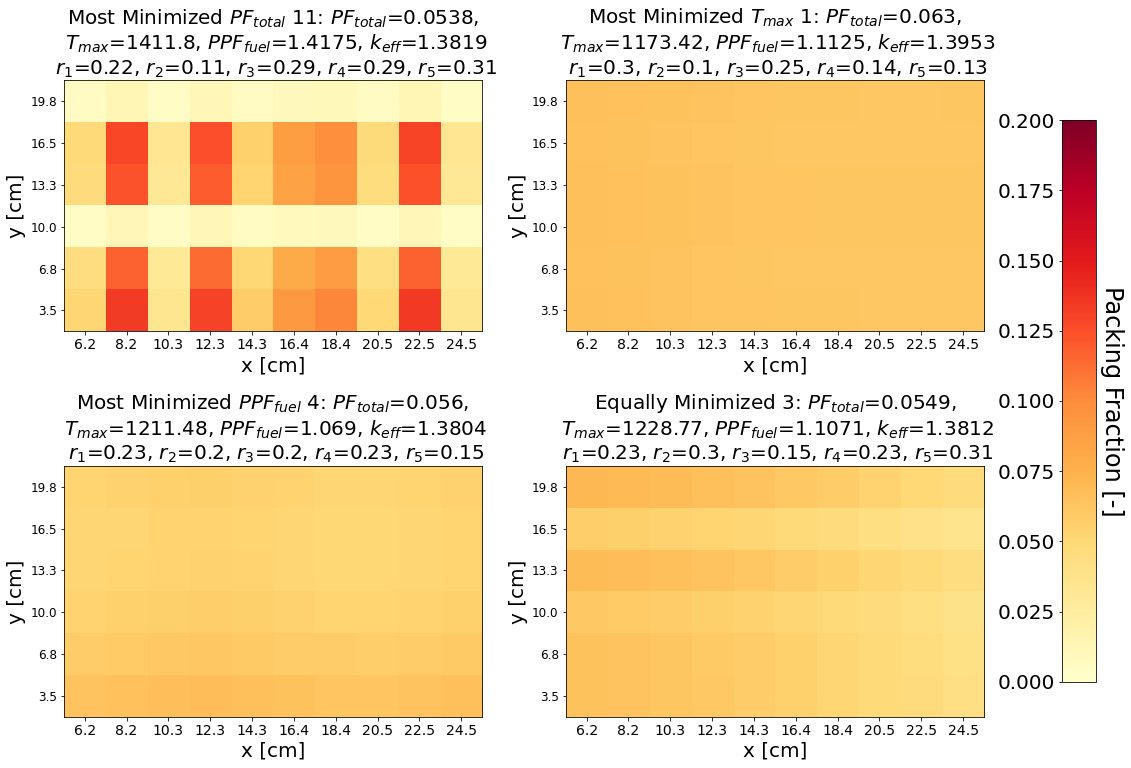
\includegraphics[width=0.8\linewidth]{../docs/figures/assem-obj-3-all-distr-most-minimized.png} 
        \caption{Simulation a-3b Pareto Front's TRISO Distributions.}
    \end{figure}
\end{frame}

\begin{frame}
    \frametitle{AHTR One-Third Assembly Simulation a-3b Results}
    \begin{figure}
        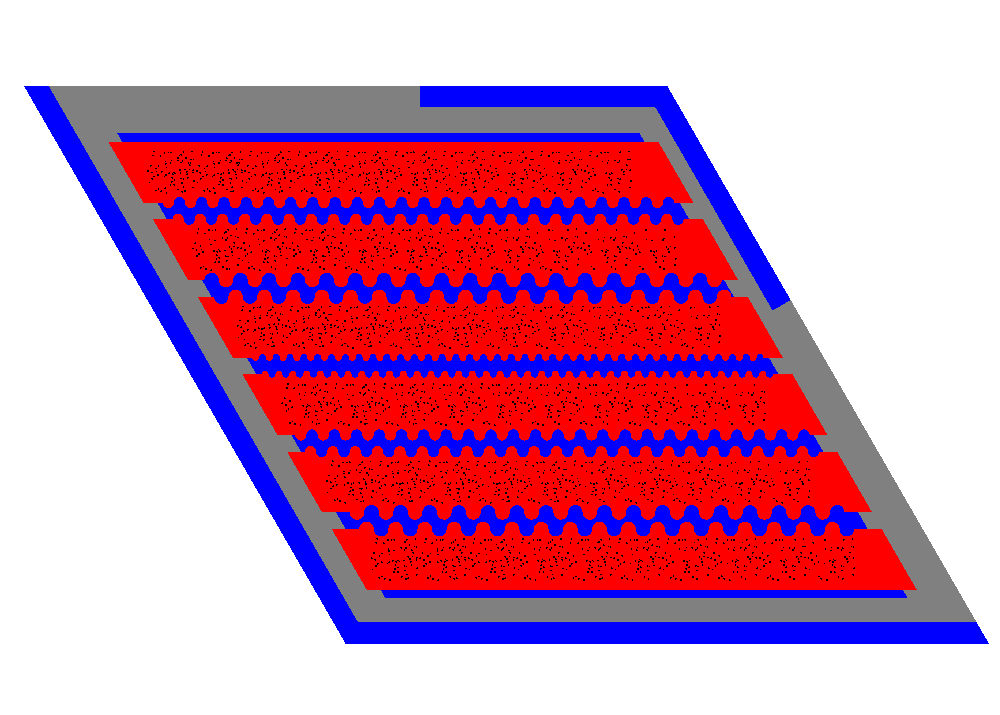
\includegraphics[width=0.75\linewidth]{../docs/figures/assem-obj-3-all-min-all.png} 
        \caption{Simulation a-3b: one-third assembly model that equally minimized all 
        objectives (reactor model 2).}
    \end{figure}
\end{frame}

\begin{frame}
    \frametitle{Multi-Objective Optimization Major Takeaways}
    The multi-objective optimization simulations successfully found a \textbf{wide 
    spread of reactor models on their Pareto fronts}. 

    \vspace{0.2cm}
    The reactor models on the Pareto fronts have \textbf{different $PF_{total}$, 
    TRISO distributions, and coolant channel shapes}, depending on the extent 
    each objective is minimized due to the nature of multi-objective
    optimization that results in a \textbf{tradeoff between objectives}. 

    \vspace{0.3cm}
    \textbf{Minimize $T_{max}$ objective} 
    \begin{itemize}
        \item Continues to flatten TRISO distribution 
        \item Maximize radius values of FliBe channels located near temperature peaks 
    \end{itemize}

    \textbf{Minimize $PF_{total}$ and $PPF_{fuel}$} 
    \begin{itemize}
    \item These two objectives influence each other to have unexpected TRISO
    distributions at different $PF_{total}$ values
    \end{itemize} 

\end{frame}

\begin{frame}
    \frametitle{ROLLO Tool + AHTR Optimization Simulations: Summary}
    \begin{block}{I Successfully Completed AHTR Optimization for Non-conventional Designs
    Research Objectives}
    \begin{itemize}
        \item I developed \acrfull{ROLLO} tool that enables generative reactor design
        optimization with evolutionary algorithms 
        \item I demonstrated ROLLO's application on AHTR optimization for spatially variant 
        fuel distributions and wavy coolant channels
    \end{itemize}    
    \end{block}
    \begin{block}{Major Takeaways}
        \begin{itemize}
            \item Results demonstrate ROLLO's success in conducting a multi-objective 
            global search of the large AHTR design space to find optimal reactor models 
            that satisfy all the objectives
            \item Once the ROLLO search is complete, reactor designers gain a better 
            intuition of the model's reactor physics and can view the narrower reactor 
            design space that meets their defined objectives
        \end{itemize}
    \end{block}
\end{frame}